\documentclass{ucalgarythesis}
  
%% Packages
\usepackage[utf8]{inputenc}
\usepackage{url} % Breaks up urls
\usepackage{amssymb,amsthm,amsmath,upgreek,siunitx,units} % Better math symbols
\usepackage{titlesec} % Remove chapter headings
\usepackage{setspace} % Line spacing
\usepackage{graphicx} % Graphics
\usepackage{subfig} % Insert figures side by side
\usepackage{array} % Table spacing
\usepackage[font={small}]{caption} % Small font in figure and table captions
\usepackage{color} % Colors
\usepackage[table]{xcolor} % Table color
\usepackage{float} % Floating figures and tables
\usepackage{chemformula} % Chemical formulas
\usepackage{enumitem} % Lists
%%%%%%%%%%%%%%%%%%%%%%%%%%%%%%%%%%%%%%%%%%%%%%%%%%%%%%%%%%%%%%%%%%%%%%%%%%%%%%%%%%%%%%%%%%%%%%%%%%%


%%  User-defined commands
\titleformat{\chapter}[display]
{\normalfont\bfseries}{}{0pt}{\Huge}
\setstretch{1.4}
\setlength{\parindent}{0pt}
\newcommand{\eqname}[1]{\tag*{#1}} % Tag equation with name
\newcolumntype{P}[1]{>{\centering\arraybackslash}p{#1}} % Table Spacing
\renewcommand{\labelitemii}{$\circ$} % Second bullet symbol
\renewcommand{\labelitemiii}{$\cdot$} % Third bullet symbol
\newcommand\ddfrac[2]{\frac{\displaystyle #1}{\displaystyle #2}} % Less cramped fractions
%%%%%%%%%%%%%%%%%%%%%%%%%%%%%%%%%%%%%%%%%%%%%%%%%%%%%%%%%%%%%%%%%%%%%%%%%%%%%%%%%%%%%%%%%%%%%%%%%%%


%% Colors
\definecolor{greenOverleaf}{RGB}{19, 138, 7}
\definecolor{orangeRed}{RGB}{255, 90, 90}
\definecolor{Gray}{gray}{0.85}
%%%%%%%%%%%%%%%%%%%%%%%%%%%%%%%%%%%%%%%%%%%%%%%%%%%%%%%%%%%%%%%%%%%%%%%%%%%%%%%%%%%%%%%%%%%%%%%%%%%




\begin{document}
%% Title Page
\frontmatter
\makethesistitle
\newpage
%%%%%%%%%%%%%%%%%%%%%%%%%%%%%%%%%%%%%%%%%%%%%%%%%%%%%%%%%%%%%%%%%%%%%%%%%%%%%%%%%%%%%%%%%%%%%%%%%%%


%% Executive Summary
\chapter{Executive Summary}
According to ASHRAE, Canada consumes approximately 347 PJ of energy, or 9.5 billion cubic meters of natural gas equivalent for residential and commercial hot water applications on an annual basis. The dependency on this “bridge” fossil fuel leads to approximately ~18 megatons of $CO_2$
equivalent emissions. With the current urgency of altering energy practices to combat climate change, and Canada’s initiative of becoming a net-zero economy by 2050, the need to adopt cleaner technologies has become paramount.

\medskip
Direct expansion solar assisted heat pump (DX-SAHP) systems have the potential to provide the heat load required for domestic hot water ($\sim$55\textdegree C) sustainably and with minimum emissions. Contrary to conventional air-source heat pumps, DX-SAHP utilize a solar thermal
collector to evaporate the working fluid using less energy in the process thereby achieving a higher coefficient of performance ($COP$). With Calgary’s cold climate and the highest solar potential in Canada of about 2396 hours or sunlight available 333 days a year, such a system would make technical and economic sense. In this paper, the design, fabrication, and testing of DX-SAHP system for cold climates is presented. The system consists of a $2m^2$ collector made from an aluminum plate with a serpentine copper tube of $5/16$ in diameter.
Refrigerant from the evaporator exchanges heat with water from a $178L$ domestic hot water tank through an intermediate condensing heat exchanger coil. After condensation the refrigerant is throttled to the evaporator pressure to restart the cycle.

\medskip 
A ranking matrix was used to select an appropriate working fluid with emphasis on safety, performance, and environmental impact such as the Ozone Depletion Potential (ODP) and Global Warming Potential (GWP) of the refrigerant. As such, R134a was selected as a suitable refrigerant owing to the higher Coefficient of Performance (COP) and its wide availability
compared to other refrigerants, however drop-in replacements for the system will be considered.

\medskip
A mathematical model representing the system was developed by combining the Hottel-Whillier equation for the solar collector and a control volume analysis using the first law of thermodynamics for heat pump cycle. The solution was obtained iteratively using MATLAB coupled with CoolProp and meteorological weather data to determine the theoretical values of
sequestered heat, collector efficiency, and the COP of the system. Theoretical results showed that a $COP$ in the range of $3.4 - 4.5$ was achievable. With the promising theoretical results, an experimental test setup was constructed to determine the long-term performance of a DX-SAHP under local climatic conditions. Temperature, pressure, and flow data were obtained using an Arduino microcontroller-based Data Acquisition system (DAQ). Moreover, an economic analysis of the system, including projected cost of adoption,
estimated energy savings, and payback period are discussed.

\newpage
%%%%%%%%%%%%%%%%%%%%%%%%%%%%%%%%%%%%%%%%%%%%%%%%%%%%%%%%%%%%%%%%%%%%%%%%%%%%%%%%%%%%%%%%%%%%%%%%%%%

 
%% Acknowledgements
\chapter{Acknowledgements}  
The Direct Expansion Solar Assisted Heat Pump project is supported by the Department of Mechanical and Manufacturing Engineering at the University of Calgary. The authors would like to acknowledge Dr. Aggrey Mwesigye, Dr. Simon Li, and Dr. Ron Hugo for providing their technical expertise in support of the development of this project. The authors would like to express their sincere gratitude for the additional sponsorship from industry professional Joshua Boles and his team at Emerson for providing technical assistance concerning the assembly of the refrigeration cycle of the Direct Expansion Solar Assisted Heat Pump system . The authors are also grateful to industry professional David Barret of Klass Mechanical for providing insights crucial to the successful manufacturing of the Direct Expansion Solar Assisted Heat Pump system. Special thanks to Frank of FN insulations for sponsoring the mineral wool insulation for the solar thermal collector.
\newpage
%%%%%%%%%%%%%%%%%%%%%%%%%%%%%%%%%%%%%%%%%%%%%%%%%%%%%%%%%%%%%%%%%%%%%%%%%%%%%%%%%%%%%%%%%%%%%%%%%%%

    
%% Table of Contents
\tableofcontents
\newpage
%%%%%%%%%%%%%%%%%%%%%%%%%%%%%%%%%%%%%%%%%%%%%%%%%%%%%%%%%%%%%%%%%%%%%%%%%%%%%%%%%%%%%%%%%%%%%%%%%%%


%% List of Figures
\listoffigures
\newpage
%%%%%%%%%%%%%%%%%%%%%%%%%%%%%%%%%%%%%%%%%%%%%%%%%%%%%%%%%%%%%%%%%%%%%%%%%%%%%%%%%%%%%%%%%%%%%%%%%%%

  
%% List of Tables
\listoftables
\newpage
%%%%%%%%%%%%%%%%%%%%%%%%%%%%%%%%%%%%%%%%%%%%%%%%%%%%%%%%%%%%%%%%%%%%%%%%%%%%%%%%%%%%%%%%%%%%%%%%%%%

  
%% List of Symbols and Variables
\chapter{List of Symbols and Variables}      
\vspace{-2mm}

\textbf{Greek Letters}
\vspace{-7mm}
\begin{tabbing}
    \textbf{}\=\\
    \addsymbol \mbox{$\alpha$}: {absorbance}
    \addsymbol \mbox{$\alpha_L$}: {linear expansion coefficient $[1/K]$}
    \addsymbol \mbox{$\beta$}: {tilt angle of collector}
    \addsymbol \mbox{$\delta$}: {absorber plate thickness [m]}
    \addsymbol \mbox{$\varepsilon$}: {emissivity}
    \addsymbol \mbox{$\mu$}: {viscosity $[Pa\cdot s]$}
    \addsymbol \mbox{$\nu$}: {kinematic viscosity $[m^2/s]$}
    \addsymbol \mbox{$\rho$}: {density $[kg/m^3]$}
    \addsymbol \mbox{$\sigma$}: {Boltzmann's constant}
    \addsymbol \mbox{$\uptau$}: {transmittance} 
\end{tabbing}
\vspace{-3mm}

\textbf{Capital Letters}
\vspace{-7mm}
\begin{tabbing}
    \textbf{ }\=\\
    \addsymbol \mbox{$A$}: {collector area $[m^2]$}
    \addsymbol \mbox{$C_b$}: {bond conductance $[W/mK]$}
    \addsymbol \mbox{$C_p$}: {thermal capacitance of circulating fluid}
    \addsymbol \mbox{$D$}: {outside pipe diameter $[m]$}
    \addsymbol \mbox{$D_i$}: {inside pipe diameter $[m]$}
    \addsymbol \mbox{$E$}: {Young's Modulus of Elasticity $[N/m^2]$}
    \addsymbol \mbox{$F'$}: {collector efficiency factor}
    \addsymbol \mbox{$FR$}: {collector heat removal factor}
    \addsymbol \mbox{$F_cr$}: {critical buckling load $[N]$}
    \addsymbol \mbox{$I$}: {irradiance $[W/m^2]$}
    \addsymbol \mbox{$K_L$}: {loss coefficient}
    \addsymbol \mbox{$L_c$}: {collector length $[m]$}
    \addsymbol \mbox{$L_p$}: {length of pipe $[m]$}
    \addsymbol \mbox{$P_e$}: {Pressure drop due to elbows $[Pa]$}
    \addsymbol \mbox{$P_f$}: {pressure drop due to friction $[Pa]$}
    \addsymbol \mbox{$Q$}: {heat transfer $[W]$}
    \addsymbol \mbox{$Re$}: {Reynolds number}
    \addsymbol \mbox{$T$}: {temperature $[K]$}
    \addsymbol \mbox{$U$}: {heat loss coefficient $[W/m^2K]$}
    \addsymbol \mbox{$V_w$}: {wind speed $[m/s]$}
    \addsymbol \mbox{$W$}: {tube centre to centre distance $[m]$}
\end{tabbing}
\vspace{-3mm}

\textbf{Lowercase Letters}
\vspace{-7mm}
\begin{tabbing}
    \textbf{ }\=\\
    \addsymbol \mbox{$e$}: {absolute pipe roughness [m]}
    \addsymbol \mbox{$f$}: {friction factor}
    \addsymbol \mbox{$g$}: {gravity $[m/s^2]$}
    \addsymbol \mbox{$h$}: {heat loss coefficient}
    \addsymbol \mbox{$h_{c,p-c}$}: {convection heat transfer coefficient between absorber plate and cover}
    \addsymbol \mbox{$h_{fi}$}: {heat transfer coefficient between fluid and tube wall}
    \addsymbol \mbox{$h_{w}$}: {convection heat transfer coefficient between the cover and the ambient}
    \addsymbol \mbox{$k$}: {conductivity}
    \addsymbol \mbox{$k_{eff}$}: {effective length}
    \addsymbol \mbox{$\dot m$}: {mass flow rate of refrigerant $[kg/s]$}
    \addsymbol \mbox{$r$}: {radius of gyration $[m]$}
    \addsymbol \mbox{$w$}: {velocity of fluid $[m/s]$}
    \addsymbol \mbox{$z$}: {height $[m]$}
\end{tabbing}
\vspace{-3mm}

\textbf{Subscripts}
\vspace{-7mm}
\begin{tabbing}
    \textbf{ }\=\\
    \addsymbol \mbox{$a$}: {ambient}
    \addsymbol \mbox{$c$}: {collector }
    \addsymbol \mbox{$g$}: {glazing}
    \addsymbol \mbox{$I$}: {insulation}
    \addsymbol \mbox{$i$}: {inlet of refrigerant}
    \addsymbol \mbox{$k$}: {conductivity}
    \addsymbol \mbox{$L$}: {heat out}
    \addsymbol \mbox{$p$}: {plate}
    \addsymbol \mbox{$pm$}: {plate mean}
    \addsymbol \mbox{$U$}: {heat in}
\end{tabbing}
\newpage
%%%%%%%%%%%%%%%%%%%%%%%%%%%%%%%%%%%%%%%%%%%%%%%%%%%%%%%%%%%%%%%%%%%%%%%%%%%%%%%%%%%%%%%%%%%%%%%%%%%


%% Content
\mainmatter

\chapter{Project Overview}

\section{Background and Motivation}

Climate change is a growing concern due to the effects that global warming has on the environment. As the population of the world increases, the energy demand will increase in turn. Due to the reliance on fossil fuels, this will only increase the amount of greenhouse gases that is produced into the atmosphere. This is why it is important to explore alternative energies that are relatively “greener” in comparison to the standard fossil fuels that are mainly used.

\medskip
A major sector where energy can be saved is domestic hot water heating. 19.3\% of the residential energy usage in Canada is from water heating [2]. This statistic can be improved with the implementation of technology that uses other sources of energy to provide water heating. This project focuses on a Direct Expansion Solar Assisted Heat Pump (DX-SAHP), which is an example of a technology that can be used in place of natural gas for heating. The DX-SAHP combines the benefits of a heat pump with the abundance of solar energy that we receive.

\medskip
Unlike an Air Source Heat Pump (ASHP), the DX-SAHP uses a combination of solar energy and the ambient temperature to evaporate the refrigerant, improving the performance and making it viable for areas with a colder climate. The use of solar energy in conjunction with the heat pump reduces the amount of electricity that is needed for a standard heat pump to generate hot water.

\newpage
\begin{figure}[ht]
    \centering
    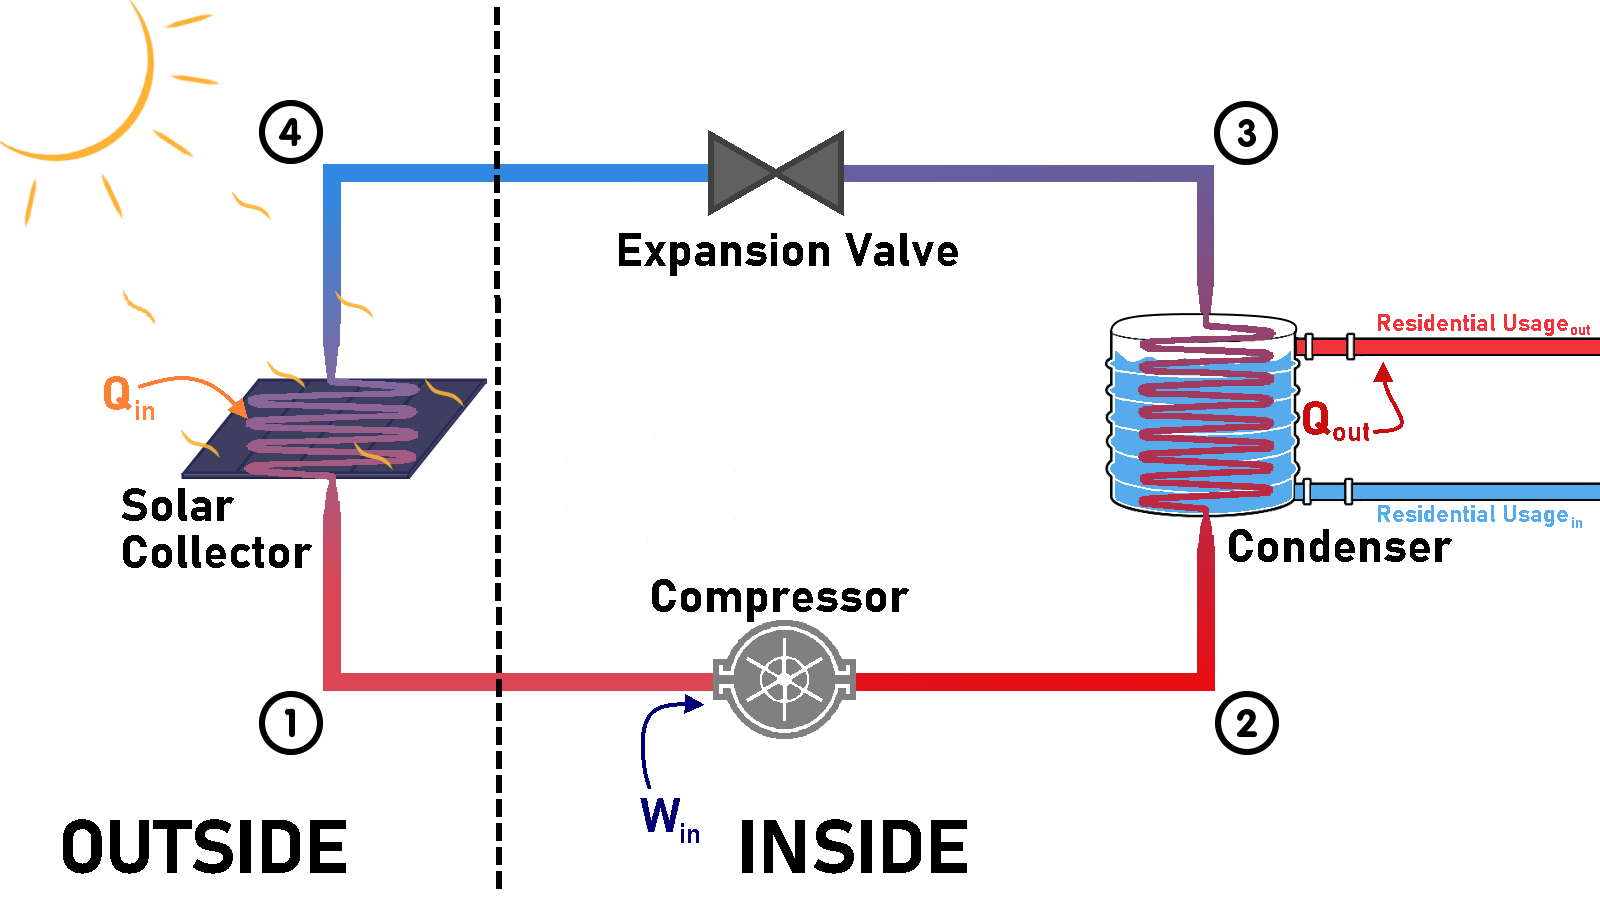
\includegraphics[width=\textwidth]{images/schematic.png}
    \caption{DX-SAHP Schematic}
\end{figure}
\medskip
The solar collector is what will be used instead of a traditional evaporator in the DX-SAHP. The collector is heated up, due to it being in direct sunlight, and thus it heats up and evaporates the refrigerant running below it. Ambient temperatures play a critical role in the performance of a heat pump with a solar collector. This is due to the solar collector directly being affected by how much irradiance, the amount of light striking a surface, is available. To design a collector for colder climates, where perhaps less irradiance is available, there must be key considerations that are considered. Additionally, other required components must be matched to the demand and to the solar collector size.

\section{Problem Statement}
The current state of heating in Alberta is overly reliant on natural gas and the technology that is currently being used to heat domestic water is contributing to the increase in global temperatures via greenhouse gas emissions. DX-SAHP can be used to phase out natural gas heaters by using the sun as an energy source instead. Therefore, a DX-SAHP can be designed that can heat an average household of 3 people within the Calgary region.

\section{Design Requirements}
The goal of this capstone is to design a DX-SAHP that can heat 225L of domestic hot water to a household of 3 people. This number was calculated from the information from the Government of Canada stating that the average Canadian uses 75L of hot water a day [2]. Knowing this, a DX-SAHP will be designed and manufactured. The effort will be mainly focused on optimizing the area of the collector while reducing the heat losses from convection and radiation. Component matching analysis and selecting a compatible compressor, condenser, and electronic expansion valve is necessary so that it is system functions properly. This heat pump must be equipped with all the necessary controls and data acquisition systems. Afterwards a working model will be made in order to be functional within Calgary and an economic and environmental analysis will be conducted to justify the proposed system.

\medskip
To determine the sizing of the DX-SAHP initial parameters must be set.

\medskip
Statistics Canada states that the average Canadian household occupies 2.47 members, and the average Canadian uses 75L of hot water per day [3]. For the purposes of the DX-SAHP, it will be assumed that a domestic household of 3 people will require 225L of hot water per day. The hot water will be required to exit the system at a temperature of 50\textdegree C for residential use to avoid bacteria buildup in the water tank such as legionella. 

\medskip
The municipal water supply differs in temperature depending on the time of year. When it is winter, municipal line comes in at 10\textdegree C unlike in the summer when it comes in at 20\textdegree C. This is an important parameter to be considered when quantifying what heat load the heat pump will have to supply.

\medskip
To validate and maintain quantifiable design goals, the project will be considered successful if it is able to sustain 225L of water at 50\textdegree C while maintaining a coefficient of performance ($COP$) greater than 2.3. This means the DX-SAHP must be able to provide the following heat loads.

\smallskip
\begin{align}
    Q_L = 225L \times \frac{1000g}{1L} \times 4.18\frac{J}{g\SI{}{\celsius}}\times (\SI{50}{{\celsius}} - \SI{10}{{\celsius}}) = 37,620kJ
    \\\eqname{Heat Load Required during Winter Conditions}
\end{align}

\begin{align}
    Q_L = 225L \times \frac{1000g}{1L} \times 4.18\frac{J}{g\SI{}{\celsius}}\times (\SI{50}{\celsius} - \SI{20}{\celsius}) = 28,215kJ
    \\\eqname{Heat Load Required during Summer Conditions}
\end{align}

\chapter{Conceptual Design}

\section{Background Research}

The most common water heater is the storage tank water heater. The way it functions is by heating up water that will be stored within a storage tank. This is most conventional since it is easy and cheap to install when comparing it to other water heaters. The limiting factor is that it is limited by the size of the storage tank. It may take a while for the hot water to be heated again if it runs out.

\medskip
Another type of water heater that is used is an Air Source Heat Pump (ASHP). What makes this heat pump unique is that it uses the heat within the air to heat the water. All it needs is a little bit of electricity to power the system. This makes the ASHP two to three times more efficient than most water heaters \cite{heat_pump_water_heaters}. The major drawback is that it needs to take heat from the air, therefore it is not suitable for basements or colder climates.

\begin{figure}[ht]
    \centering
    \subfloat[\centering Storage Tank Water Heater {\cite{water_heater_img1}}] {{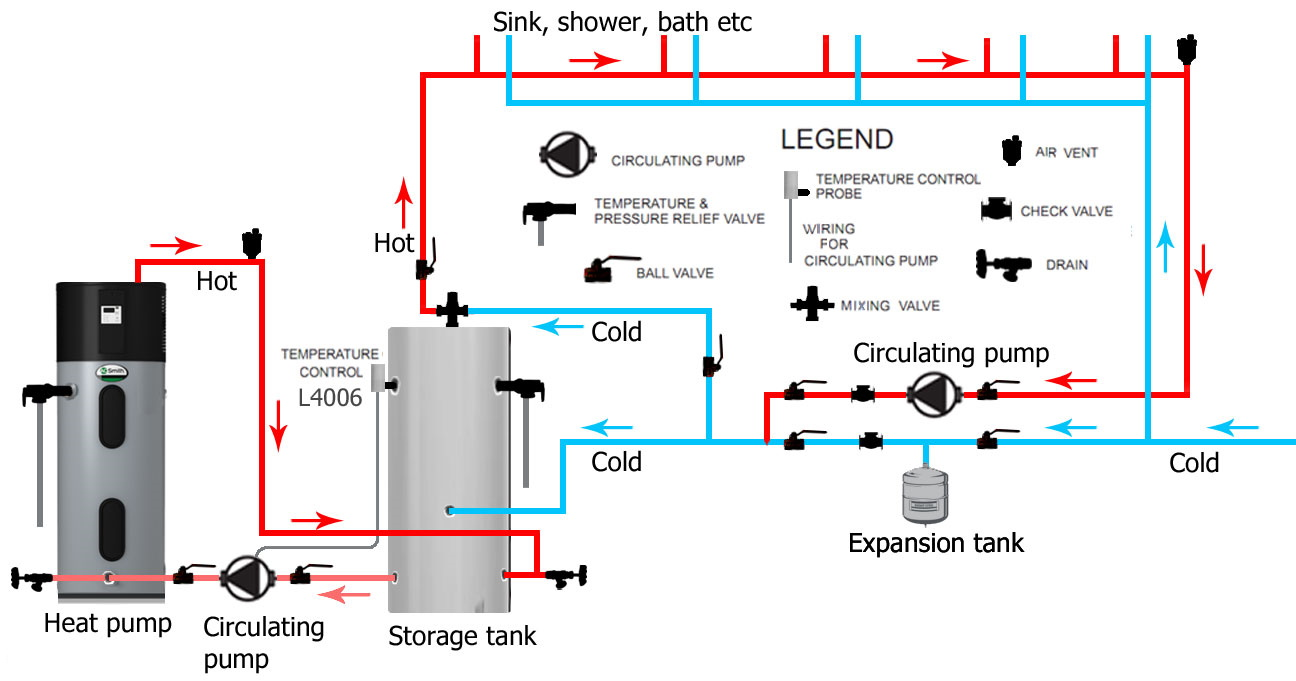
\includegraphics[width=7.7cm]{images/storage_tank_water_heater.jpg}}}
    \qquad
    \subfloat[\centering Air Source Heat Pump Water Heater {\cite{water_heater_img2}}] {{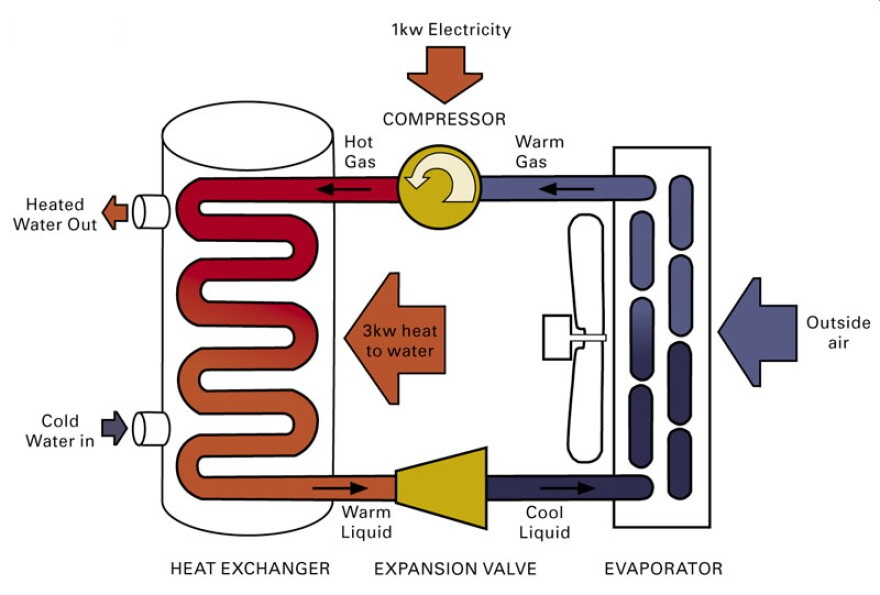
\includegraphics[width=7.7cm]{images/air_source_heat_pump.jpg}}}
    \caption{Conventional Water Heaters}
\end{figure}

\smallskip
Unlike the ASHP, the DX-SAHP uses solar energy to provide the heat needed to heat the water. When comparing Figure 2.2 with Figure 1.1, a solar collector is used instead of an evaporator. This gives all the benefit of an Air Source Heat Pump with the additional benefit of working in colder climates since the sun can provide enough energy to heat the water.

\medskip
When designing a DX-SAHP, it is important to consider the irradiance available in the area. Irradiance is the amount of energy received from the sun within an area. As seen in Table 1, the amount of sun Calgary receives is drastically different between the winter and summer data sets.

\medskip
Winter months are defined from October to March in Table 2.1 while summer is between April to September. The justification behind choosing those date ranges is that it makes use of the entire year, and it is split between when Calgary has the most daylight hours versus the least. It also happens to line up with the solstices.

\medskip

\begin{table}[H]
\centering
\caption{Calgary Irradiance Data}
\rowcolors{2}{gray!20}{white}
\begin{tabular}{|P{10mm}|P{70mm}|P{70mm}|}
    \hline
    \rowcolor{orangeRed}
    Hour &  Average Winter Irradiance Data $(W/m^2)$ & Average Summer Irradiance Data $(W/m^2)$ \\
    \hline
    1 & 0 & 0 \\
    2 & 0 & 0 \\
    3 & 0 & 0 \\
    \cite{heat_pump_water_heaters} & 0 & 0 \\
    5 & 0 & 1.398907104 \\
    6 & 0 & 12.99453552 \\
    7 & 0.510989011 & 76.3715847 \\
    8 & 7.736263736 & 182.0710383 \\
    9 & 54.40659341 & 327.442623 \\
    10 & 149.6538462 & 445.6065574 \\
    11 & 229.7857143 & 557.2896175 \\
    12 & 289 & 612.0601093 \\
    13 & 316.7087912 & 629.9289617 \\
    14 & 301.6868132 & 587.7923497 \\
    15 & 252.4285714 & 539.8196721 \\
    16 & 178.3241758 & 474.3715847 \\
    17 & 86.85714286 & 374.3879781 \\
    18 & 29.04395604 & 252.4043716 \\
    19 & 3.708791209 & 142.9016393 \\
    20 & 0 & 44.86885246 \\
    21 & 0 & 4.256830601 \\
    22 & 0 & 0 \\
    23 & 0 & 0 \\
    24 & 0 & 0 \\
    \hline
\end{tabular}
\end{table}

\medskip
\section{Sponsor Requirements}
The sponsor's requirement for this capstone project was the design of a  DX-SAHP system that can satisfy the domestic hot water demand of the average Canadian household (~225L) of hot water per day \cite{stats_canada}.The system had to be disassemble, which was considered through the fabrication of a 3-part support frame, and through the incorporation of valves between the HVAC subcomponents. 

\medskip
\section{Collector Type Selection}

There are three types of solar collectors that are commonly used in the market; they are flat plate collectors, evacuated tube collectors, and concentrating collectors. Each comes with their own benefits and drawbacks.

\medskip
Flat plate collectors consist of a flat absorber plate that is orientated towards the sun. They use both direct and diffuse solar radiation and normally do not require a tracking system. Their main applications are solar water heating, heating for buildings, air conditioning and heat for industrial processes \cite{solar_thermal_energy}.

\medskip
In contrast, evacuated tube collectors consist of several rows of parallel transparent glass tubes which have the working fluid flowing within it. The glass tubes are cylindrical in shape which results in the sunlight always being perpendicular to the heat absorbing tubes. This is a major benefit since this collector can be used when the sun is low in the sky or on cloudy days and they are particularly useful in colder climates.

\medskip
Concentrating collectors are more suited for systems that require higher temperatures than what is achievable with a flat collector. The concentrating collector can be optimized by decreasing the area of heat loss when comparing it to flat plate collectors. This is done by placing an optical device between the source of radiation and the surface. A disadvantage that this technology has is that a sun tracking system is required to always maximize the incident radiation. This tracking system increases the overall cost of the collector and leads to additional maintenance which is why it was not considered at all for this project \cite{solar_thermal_energy}.

\medskip
When comparing flat plate collectors with evacuated tubes, there are several categories that can be considered. When comparing costs, evacuated tubes are around 10-15\% more expensive than flat plate. This was important to consider due to the limited budget that this project has \cite{flat_plate}. Another important area that needs to be looked at would be how the collector can handle snow. Since there will be no tracking system for our design, there will be no way to shake off the snow, so the collector must remove it passively. The benefit of a flat plate collector is that snow can shed easily unlike with evacuated tubes in which it can get stuck due to the tubes creating a strong vacuum \cite{flat_plate}.

\medskip
Both flat plate and solar collectors are excellent at heating water. The main question that needs to be asked when selecting the collector type is how much water needs to be heated to the desired temperature. Evacuated tubes are great for colder climates since they can heat water up to 121\textdegree C but it has the tendency to overheat. Therefore, evacuated tubes are more commonly used for commercial rather than domestic purposes. Unlike evacuated tubes, flat plate collectors can heat water up to 82\textdegree C which means that it is has smaller chance of overheating. This temperature range is suitable for domestic hot water usage \cite{flat_plate}.

\medskip
When looking at all the parameters, the flat plate collector was selected instead of the evacuated tube or concentrating collector. Although the evacuated tube collector works better in colder climates than the flat plate collector, it was excessive in terms of both cost and design work for domestic water heating. The flat plate satisfies many requirements for a collector in colder climates, and it is the recommended collector for domestic water heating \cite{flat_plate}. Therefore, for the design, the flat plate collector was chosen.

\section{Refrigerant Selection}

A refrigerant is a working fluid used in the thermodynamic cycle of a heat-pump, where the fluid will undergo multiple phase changes from liquid to vapor and vice versa, throughout the system cycle. One of the first components in a heat pump, which must be determined early on, is the refrigerant. To determine which components (i.e., compressor, condenser, and expansion valve) will be used in the DX-SAHP, the working fluid must be selected. Although there were many refrigerants to choose from, the list was drastically cut down after considering multiple criteria. These criteria looked at the environmental acceptability, safety, application, performance, and the economics associated with various refrigerants.

\medskip
The Ozone Depletion Potential (ODP) is a measure of a refrigerant’s ability to damage the ozone layer relative to CFC-11 with an ODP of 1. Emissions from CFC’s (chlorofluorocarbons), HCFC’s (hydrochlorofluorocarbons), and other synthetic chemicals which created an “ozone hole” over the South Pole \cite{ozone_layer} have led to the Montreal Protocol on Substances that deplete the Ozone layer \cite{odp} – a global agreement made to phase out ozone-depleting substances. For the DX-SAHP, only refrigerants with an ODP equal to zero were considered.

\medskip
The Global Warming Potential (GWP) is the next major criterion regarding environmental acceptability. This is a metric measuring the energy of emissions, which one ton of a specific gas will absorb relative to the emissions of one ton of carbon dioxide (\ch{CO2}) over a hundred-year period \cite{gwp}. For example, a refrigerant with a GWP of 1430 will have 1430 times the global warming potential of \ch{CO2} over 100 years. In 2016, the Kigali amendment was made to the Montreal Protocol \cite{montreal_protocol}, proposing a complete phase down of HFCs by 2047 due to their high global warming potential. Furthermore, the European Union \cite{hfcs} took action to place market prohibitions on gases with a GWP greater than 750 in air-conditioning systems by 2025. Therefore, the considered refrigerants had to have a GWP below 750.

\medskip
Refrigeration cycles have three distinct applications: high temperature (comfort conditioning), medium temperature (food refrigeration), and low temperature (transport refrigeration). Domestic water heating falls into high temperature comfort conditioning applications. The most widely used refrigerant in these applications has been R-134A and R-134A. Due to the high SEER (Seasonal Energy Efficiency Ratio) ratings of R-134A compared to other refrigerants, it, along with R-410A, has dominated the air conditioning market for components. However, due to R-134A’s high GWP of 1430, refrigerants with similar thermodynamic properties used as replacements for the eventual phase down of R-134A were explored.

\newpage
Following the ASHRAE Standard 34 refrigerant safety classification, most refrigerants in use currently pose a very low toxicity and flammability threat – giving an ASHRAE safety designation of A1. Following the ASHRAE Standard 34 \cite{ashrae_safety} refrigerant safety classification, most refrigerants in use currently pose a very low toxicity and flammability threat – giving an ASHRAE safety designation of A1. ASHRAE Standard 34 assigns refrigerants to two toxicity (A or B), and four flammability classes (1, 2, 2L, 3). The safety designations for refrigerants are as follows:

\begin{itemize}[itemsep=3mm, parsep=-1mm]
\item Class A (Low Toxicity)
    \begin{itemize}
        \item Occupational exposure limit is 400ppm or greater
    \end{itemize}
\item Class B (High Toxicity)
    \begin{itemize}
        \item Occupational exposure limit is less than 400ppm.
    \end{itemize}
\item Class 1 (No flame propagation)
    \begin{itemize}
        \item No flame propagation at 60\textdegree C and atmospheric pressure.
    \end{itemize}
\item Class 2L (Low flammability)
    \begin{itemize}
        \item Flame propagation at 60\textdegree C and atmospheric pressure.
        \item Lower Flammability Limit $> 0.10kg/m^3$ and Heat of Combustion $< 19,000 kJ/kg$
        \item Burning velocity <= 10cm/s at 23\textdegree C
    \end{itemize}
\item Class 2 (Flammable)
    \begin{itemize}
        \item Flame propagation at 60\textdegree C and atmospheric pressure.
        \item Lower Flammability Limit $> 0.10kg/m^3$ and Heat of Combustion $< 19,000 kJ/kg$
    \end{itemize}
\item Class 3 (High flammability)
    \begin{itemize}
        \item Flame propagation at 60\textdegree C and atmospheric pressure.
        \item Lower Flammability Limit $<= 0.10kg/m^3$ or Heat of Combustion $< 19,000 kJ/kg$
    \end{itemize}
\end{itemize}

\medskip
Because the system was designed for a residential water heating supply, only refrigerants designated in Class A toxicity were used due to possibility of leakage.

\medskip
As with many design considerations in engineering, there is an equivalent exchange when reducing the global warming potential of refrigerants. A general trend can be observed in refrigerants where a lower GWP equates to a higher flammability designation; most new generation refrigerants with a GWP less than 750 have an ASHRAE safety designation of A2L. While refrigerants of Class 1 are the most desirable, Class 2L refrigerants can also be considered safe \cite{low_gwp} to use in domestic heating systems as they have a high Minimum Ignition Energy and would need to be exposed to an open flame or high energy source with sufficient concentrations to ignite.

\medskip
Although each refrigerant will result in different system efficiencies, by looking at the critical temperature of the refrigerant, a correlation can be made for both the coefficient of performance and the cooling capacity of the system. As the critical temperature of the refrigerant increases, the coefficient of performance of the system is found to increase, while the cooling capacity is found to decrease \cite{low_gwp_options}. A higher coefficient of performance will ultimately result in a lower energy bill for the end user, while a lower cooling capacity will result in a larger system. As the project location is for a cold climate in Calgary, the refrigerant must also be chosen to have a freezing point, $T_{fp} < \SI{-50}{\celsius}$. Furthermore, CoolProp \cite{cool_prop} was used to conduct the thermodynamic analysis, and therefore, refrigerants of choice must be available on the database such that the system calculations can be performed.

\medskip
Finally, the economics and procurement of the refrigerants were considered where the system will require between 3-6 pounds of charge. After contacting vendors, many refrigerants were found to have more than 3 months lead times due to COVID-19 supply chain issues, and as a result would not satisfy the project’s timeline. Many new generation refrigerants were also found to be cost-ineffective when compared to their incremental performance benefits. These refrigerants ranged from \$400 to \$3000 per their minimum selling quantities.

\medskip
A design requirements table was then created to easily compare the refrigerants as seen below.

\medskip
\begin{table}[H]
\centering
\caption{Refrigerant Criteria}
\rowcolors{2}{gray!20}{white}
\begin{tabular}{|P{23mm}|P{23mm}|P{23mm}|P{23mm}|P{23mm}|P{23mm}|}
    \hline
    \rowcolor{orangeRed}
    Refrigerant &  ODP & GWP & Alternative To & Safety Class & $T_{critical}$ (\textdegree C) \\
    \hline
    R-410A           & 0 & 2088 & R-22   & A1  & 72.13 \\
    R-717 (\ch{NH3}) & 0 & 0    & R-22   & B1  & 132.4 \\
    R-1234yf         & 0 & 4    & R-134A & A2L & 94.70 \\
    R-1234ze         & 0 & 1    & R-134A & A2L & 109.4 \\
    R-32             & 0 & 675  & R-410A & A2L & 78.40 \\
    R-454B           & 0 & 466  & R-410A & A2L & 78.10 \\
    R-454C           & 0 & 148  & R-410A & A2L & 82.40 \\
    R-455A           & 0 & 146  & R-410A & A2L & 86.60 \\
    R-466A           & 0 & 733  & R-410A & A1  & 76.50 \\
    R-515B           & 0 & 299  & R-134A & A1  & 108.7 \\
    R-290            & 0 & 3    & R-410A & A3  & 97.00 \\

    \hline
\end{tabular}
\end{table}

\medskip
After assessing these criteria, and contacting supply vendors, it was determined that R-32 was preferred refrigerant for the  DX-SAHP system. The decision was contingent upon the refrigerant’s suitability with the team’s initial selection criteria. With a zero ODP, a GWP less than 750, a critical temperature of 78.4\textdegree C, but most importantly, a procurement time of 2 months, the R-32 was determined to be the appropriate working fluid.

\medskip
Upon determination of R-32 as the working fluid for the system, the component matching phase began. Although some components were found for this refrigerant (e.g., expansion valve), when looking for a compressor compatible with R-32, and which could be procured within a reasonable time frame, component matching proved to be difficult.

\medskip
After consulting with a subject matter expert working in the heating ventilation and cooling (HVAC) sector for over 15 years, the team determined the reason for the difficulties to be that R-32 and all other similar new generation refrigerants are still considered novel to the industry. As R-134A is still dominating the air conditioning industry in North America, components for comfort cooling heat pump applications are designed around R-134A being the working fluid. However, the research was not in vain; since R-32 is the widespread refrigerant of choice in Asia and is slowly being phased in around parts of Europe as the next replacement for high GWP refrigerants, it is beneficial to have considered it as a potential working fluid for the DX-SAHP.

\medskip
Finally, although the GWP was far too high, it was still suggested to design the system using R-134A as North America has not yet caught up with the refrigerant phase down plan. Furthermore, the use of R-134A as a system refrigerant is not detrimental to the project’s environmental considerations as the final solution to avoid the use of a high GWP refrigerant is through sourcing drop-in replacements. A drop-in replacement for R-134A (such as HFO-1234yf) is a refrigerant which can simply swap R-1234yf while maintaining the same system components. This allows for the system calculations, and thus, the system components to be modeled and procured based upon R-134A as the working fluid. The advantage of taking the approach of using drop-in refrigerants is that, as new refrigerants become available, supply chain delays would not hinder the progress of the build assembly as R-134A could always be used to complete the project.

\section{HVAC Components}

\subsection{Compressor Type Selection}

For the purposes of the compressor in the DX-SAHP system, a hermetic sealed variable speed compressor was initially selected. This type of compressor operates via positive displacement and can achieve higher compression ratios per single stage of compression \cite{other_compressors}. Additionally, they are more compact and less prone to vibration.

\medskip
Hermetic compressors are widely used in domestic refrigeration systems wherein continuous maintenance cannot be ensured by the user. A hermetic compressor consists of the compressor part directly mounted on the shaft of the motor. The compressor and motor are confined together within an outer shell, reducing the potential for dust particles to access the interior and consequently impact the operation of the compressor \cite{hermetic_compressors}. With both the compressor and motor being directly coupled on the same shaft and confined within a common casing, the potential for leakage of R-134A is essentially eliminated \cite{what_hermetic_compressor}. The hermetic compressors investigated for the purpose of the DX-SAHP system were of the reciprocating and rotary types.

\medskip
The variable speed aspect of the compressor is facilitated by the adjustability of the motor speed in response to shifting power demands, thereby conserving energy. For the purposes of this analysis, the ability to control the speed of the compressor allows for the control of the pressure differential of the refrigerant, R-134A. Previously, it was considered essential to control the varying conditions at the compressor inlet to obtain a quasi-constant condensation temperature of 60\textdegree C. 

\medskip
However, due to the complexities associated with variable speed compressors such as capacity incompatibility, refrigerant incompatibility, as well as the elevated complexity of utilizing 3-phase motor capable of supporting the integration of a variable frequency drive, it was decided that a single speed compressor would be more adequate.

\medskip
Among the many choices for compressors depicted in Figure 2.2, the following design alternatives for a hermetic variable speed compressor have been taken into consideration, allowing for use in domestic water heating applications \cite{how_compressor_works} \cite{vapor_compression_refrigeration}.

\medskip
\begin{enumerate}[itemsep=3mm, parsep=-1mm]
    \item Scroll variable speed compressor \cite{scroll_compressors}
    \item Reciprocating variable speed compressor \cite{variable_speed_hermetic}
    \item Rotary screw variable speed compressor
    \item Centrifugal variable speed compressor
    \item Open motor hermetic speed compressor
\end{enumerate}

\medskip
The following figure shows common compressors and their classification.

\medskip
\begin{figure}[ht]
    \centering
    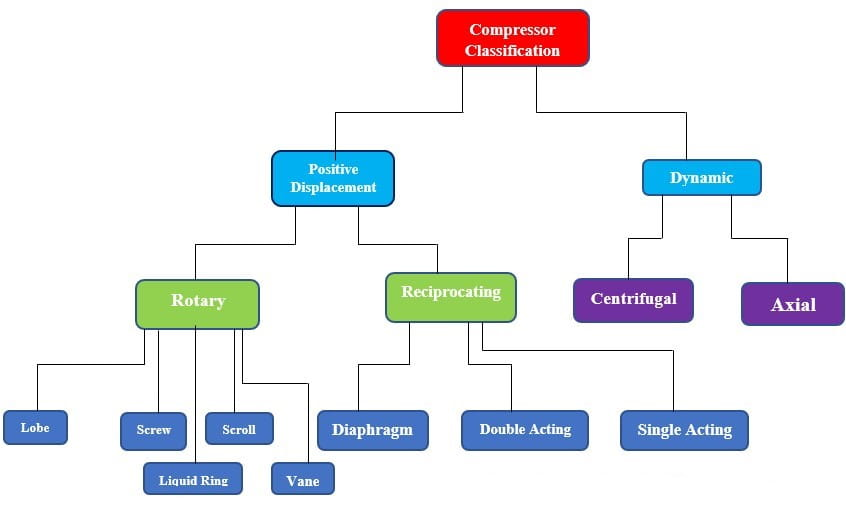
\includegraphics[width=\textwidth]{images/compressor_types.jpg}
    \caption{Compressor Classification \cite{air_compressor}}
\end{figure}

\medskip
Out of the five listed compressors, the suitable design alternative was found to be the scroll compressor as it offers the following design-specific benefits:

\medskip
\begin{enumerate}[itemsep=3mm, parsep=-1mm]
    \item lower compressor power ratings.
    \item compatible with R-134A.
    \item single phase.
    \item operate within the operating pressures of the system design parameters.
    \item operate within the evaporating temperature ranges of the system design parameters.
    \item have low sound and vibrations.
    \item longer compressor life.
    \item reduces leak potential.
    \item exhibit energy saving capabilities \cite{scroll_compressor} \cite{what_scroll_compressor}.
\end{enumerate}

\medskip
Notwithstanding, the rotary screw and reciprocating positive displacement variable speed compressors may also be used for the purposes of the DX-SAHP. However, since rotary screw compressors are more commonly used in commercial and industrial applications, they are not the most suitable alternative. Contrastingly, reciprocating compressors are commonly used in residential applications; however, they were not the preferred option due to their loud noise, limited speed and the tendency for their piston ring to wear and reduce their efficiency.

\medskip
A centrifugal type of compressor was also not the preferred alternative since these compressors are often used in industrial applications, large chillers, refineries, and plants \cite{centrifugal_compressor}. Therefore, they operate at a much higher horsepower and for higher operating pressures than required for the purpose of the DX-SAHP. Finally, the open motor variable speed hermetic compressor is not suitable as it presents a higher risk of refrigerant leakage than a sealed hermetic variable speed compressor or scroll compressor does.

\subsection{Condenser Type Selection}

Storage tank water heaters are by far the most prevalent configuration of water heaters available on the market today; however, tankless or “On-Demand” water heaters are slowly acquiring some of that market share due to their reputation of running more efficiently. For the purposes of selecting a condenser/water storage tank for the Direct Expansion Solar Assisted Heat Pump, the team considered the following factors:

\medskip
\begin{enumerate}[itemsep=3mm, parsep=-1mm, label=\roman*.]
    \item The operational time span of the evaporator/collector.
    \item The stability of meteorological conditions of the design locale.
    \item The temperature of the inlet municipal water supplied for domestic use.
\end{enumerate}

\medskip
By relying on weather station data from the Government of Canada \cite{climate_summary}, we determined the average, daily “bright sunshine hours”, to be 4.68 hours for Calgary during the winter season. These hours would support peak operation of the Solar Thermal Collector, and outside of which, the system performance may decline, and in extreme conditions, stagnate, ceasing the supply of hot domestic water in the absence of a suitable thermal mass. Assessing the stability or consistency of the meteorological conditions, such as ambient temperatures and average irradiance, the team concluded that the short operational time frame, paired with the instability of meteorological conditions and potential for inclement winter weather conditions, such as extreme subzero temperatures and collector shading due to snowfall, the DX-SAHP cannot support a tankless water heater module as a steady supply of hot water would not be guaranteed outside of optimal operational conditions. Furthermore, considering that the temperature of the supplied groundwater determines the length of the heating period in a tankless water heater, and that inlet municipal water is supplied at approximately 10\textdegree C during the winter, adopting a tankless water heater is not a feasible option for this application due to prolonged heating times. In conclusion, the team opted to adopt a coaxial condensing coil-style condenser well as an insulated water tank, which acts as a thermal mass from which emergency supply of hot water could be provisioned. Further selection considerations are highlighted in section 3.3.2 below.

\subsection{Expansion Valve Selection}

An electronic expansion valve was selected as the throttling valve in the DX-SAHP system. Throttling valves allow control of the amount of mass flow rate by adjusting the size of the flow path through the valve. The two types that were initially compared were the thermostatic valve (TXV) and the electronic expansion valve (EXV). 

\medskip
TXV’s typically use sensing bulbs to sense the temperature of the suction line. These bulbs are slightly warmer than the saturation temperature of the refrigerant and have an increase in pressure when the suction line temperature exceeds the saturation temperature. The increased pressure in the bulb indicates that more refrigerant is required to manage the system’s evaporating heat load. The opening of the valve occurs by the internal connections from the bulb to the power element. The power element consists of a diaphragm and with increasing pressure, the diaphragm is bent downwards to open the valve.

\medskip
EXV’s use an electronic controller to calculate the superheat based on the temperature and pressure at the suction line, and the outlet of the solar flat plate collector. For the controller to read the pressure and temperatures, respectively, pressure transducers and thermistors may be used. The programming of the controller controls the valve movement by either opening or closing the valve, based on the inputs read by the sensors.

\medskip
The main disadvantages of using a TXV is that if the pressure differential between the sensing bulb, combined pressure below the diaphragm, and the spring are significantly reduced, the opening and closing of the valve will be affected. Ultimately, this creates a problem for the system to operate as efficiently, mainly on the release of the mass flow rate as required for the heating load.

\medskip
Based on this, the EXV was selected as the throttling valve to be placed in the system. EXV’s offer more flexibility for system design requirements by having the ability to use the controller without needing to physically adjust the valve.
\chapter{Design Development}

\section{Collector Engineering Analysis}

\subsection{Heat Transfer Analysis}

To model the heat transfer, depicted in Figure 3.1, occurring on the surfaces of a flat plate collector, the following simplifications were made:

\medskip
\begin{itemize}[itemsep=3mm, parsep=-1mm]
    \item Performance is steady state. 
    \item Heat losses through the front and back are to the same ambient temperature.
    \item Construction is of the sheet and serpentine manifold type.
    \item Uniform flow exists within the tubes.
    \item Absorption of solar energy by the cover is insignificant insofar as it affects losses from the collector. 
    \item Temperature drop through the cover is negligible. 
    \item Heat flow through the cover is one-dimensional.
    \item The cover is opaque to infrared radiation. 
    \item Heat flow through the back insulation is one-dimensional. 
    \item The sky is considered a black body for long-wavelength radiation at the equivalent sky temperature.
    \item Temperature gradients around the tubes are negligible. 
    \item Properties of the collector are independent of temperature. 
    \item Dust, dirt, and snow buildup on the collector are negligible. 
    \item Shading of the collector absorber plate is negligible.
\end{itemize}

\medskip
\begin{figure}[H]
    \centering
    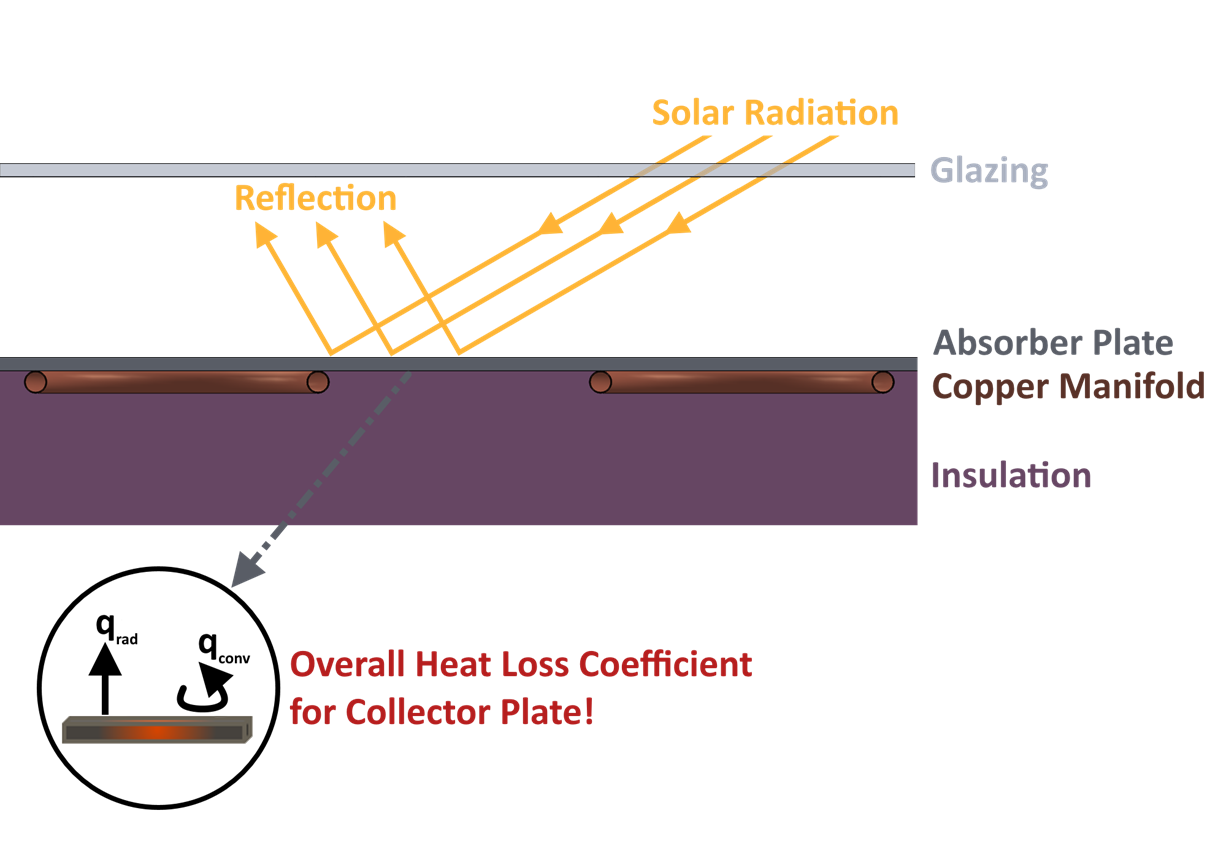
\includegraphics[width=\textwidth]{images/flat_plate_heat_transfer.png}
    \caption{Heat Transfer from a Flat Plate Collector}
\end{figure}

\medskip
The heat losses were analytically simplified by characterizing them using the thermal network depicted in Figure 3.2a. An equivalent thermal network, as shown in Figure 3.2b, can then be deduced to encompass the overall steady-state heat transfer occurring across the collector. The heat transfer analysis is derived in full detail below.

\smallskip
\begin{figure}[H]
    \centering
    \subfloat[\centering One-Cover Flat-Plate Collector] {{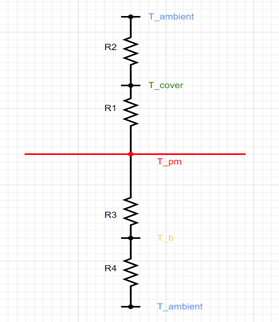
\includegraphics[width=5.2cm]{images/thermal_network.png}}}
    \qquad
    \subfloat[\centering Equivalent Thermal Network] {{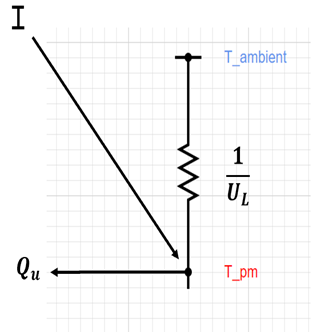
\includegraphics[width=5.2cm]{images/equivalent_thermal_network.png}}}
    \caption{Thermal Network Diagrams}
\end{figure}

\medskip
First, the top heat losses, both convective and radiative, from the absorber plate to the cover were  evaluated as follows to determine the first thermal resistance, R1:
\begin{align}
    Q_{loss, top} = h_{c, p-c}(T_{pm}-T_c) + \ddfrac{\sigma(T^4_{pm}-T^4_c)}{\frac{1}{\varepsilon_p} + \frac{1}{\varepsilon_c} - 1}
\end{align}

\begin{align}
    h_{r, p-c} = \ddfrac{\sigma(T_{pm}-T_c)(T^2_{pm}-T^2_c)}{\frac{1}{\varepsilon_p} + \frac{1}{\varepsilon_c} - 1}
\end{align}

\begin{align}
    R1 = \ddfrac{1}{h_{c, p-c} + h_{r, p-c}}
\end{align}

\bigskip
Similarly, the top heat losses, both convective and radiative, from the cover to the ambient were evaluated as follows to determine the second thermal resistance, R2:
\begin{align}
    h_{r,c-a} = \ddfrac{\sigma\varepsilon_c (T_c + T_{sky})(T_c^2 + T_{sky}^2)(T_c - T_{sky})}{(T_c - T_a)}
\end{align}

\begin{align}
    R2 = \ddfrac{1}{h_w + h_{r,c-a}}
\end{align}

\bigskip
Finally, the total top heat loss coefficient, $U_{top}$, was found to be the inverse of the summation of R1 and R2 as follows:
\begin{align}
    U_{top} = \ddfrac{1}{R1 + R2}
\end{align}

\bigskip
A useful empirical equation for $U_{top}$ was developed by Klein (1979) following the basic procedure of Hottel and Woertz (1942) and Klein (1975). This relationship fits the graphs for $U_{top}$ for mean plate temperatures between ambient and 200\textdegree C to within $\pm 0.3 W/m^2 K$ and is represented below:
\begin{align}
    U_{top} = U_{tC} + U_{tR}
\end{align}

The heat loss through convective effects, $U_{tC}$, was quantified as: 
\begin{align}
    U_{tC} = \left[  \ddfrac{M}{\left(\frac{c}{T_{pm}}\right) \left( \frac{T_{pm} - T_a}{M+f} \right)^e} + \ddfrac{1}{h_w} \right]^{-1}
\end{align}

\bigskip
Where:
\begin{align}
    f   &= (1 + 0.089h_w - 0.116h_w \varepsilon_p)(1 + 0.07866N)\\
    e   &= 0.43 \left( 1 - \ddfrac{100}{T_{pm}}\right)\\
    c   &= 520 (1 - 0.000051\beta^2)\\
    h_w &= 5.7 + 3.8V_w
\end{align}

\bigskip
The heat loss through radiative effects, $U_{tR}$, was quantified as:
\begin{align}
    U_{tR} = \ddfrac{\sigma (T_{pm}^2 + T_a^2) (T_{pm} + T_a)}{(\varepsilon_p + 0.059Mh_w)^{-1} + \frac{2M + f - 1 + 0.133\varepsilon_p}{\varepsilon_g} - M}    
\end{align}

\bigskip
Therefore:
\begin{align}
    U_{top} = \left[  \ddfrac{M}{\left(\frac{c}{T_{pm}}\right) \left( \frac{T_{pm} - T_a}{M+f} \right)^e} + \ddfrac{1}{h_w} \right]^{-1} + \ddfrac{\sigma (T_{pm}^2 + T_a^2) (T_{pm} + T_a)}{(\varepsilon_p + 0.059Mh_w)^{-1} + \frac{2M + f - 1 + 0.133\varepsilon_p}{\varepsilon_g} - M}
\end{align}

\bigskip
R3 represents the resistance to heat flow through the insulation while R4 represents the convection and radiation resistance to the environment. With appropriate back insulation, it is usually possible to assume R4 is zero and all resistance to heat flow is due to the insulation.

\medskip
The heat loss through the bottom, $U_b$, of the collector can be defined as:
\begin{align}
    U_{bottom} = \frac{1}{R} = \frac{\delta_1}{k_1}
\end{align}

The heat loss through the sides, $U_{edge}$, of the collector can be defined as:
\begin{align}
    U_{edge} = \ddfrac{Q_{edge}}{A(T_{pm} - T_a)}
\end{align}

\medskip
Where:
\begin{align}
    Q_{edge} = A_p(T_{pm} - T_a)
\end{align}

\bigskip
The total heat loss coefficient is the sum of the heat loss coefficients for the top, bottom, and sides of the collector. It can be defined as:
\begin{align}
    U_L = U_{top} + U_{bottom} + U_{edge}
\end{align}

\begin{align}
    U_L = \left[  \ddfrac{M}{\left(\frac{c}{T_{pm}}\right) \left( \frac{T_{pm} - T_a}{M+f} \right)^e} + \ddfrac{1}{h_w} \right]^{-1} + \ddfrac{\sigma (T_{pm}^2 + T_a^2) (T_{pm} + T_a)}{(\varepsilon_p + 0.059Mh_w)^{-1} + \frac{2M + f - 1 + 0.133\varepsilon_p}{\varepsilon_g} - M}\nonumber\\
    + \frac{\delta_1}{k_1} + \ddfrac{Q_{edge}}{A(T_{pm} - T_a)}
\end{align}

\bigskip
Finally, the total useful heat gain of the collector was quantified as:
\begin{align}
    Q_u = F'A_c\left[ I(\uptau_c \alpha_c) - U_L(T_{fi} - T_a) \right]
\end{align}

\bigskip
The fin efficiency represents the efficacy with which energy absorbed by the abosrber plate and the tube spacing (conceptualized as fins) is collected on the sides of the tubes for subsequent heat transfer into the working fluid:
\begin{align}
    F = \ddfrac{tanh \left[ \ddfrac{m(W-D)}{2}\right]}{\left[ \ddfrac{m(W-D}{2}\right]}
\end{align}

\newpage
Where:
\begin{align}
    m = \sqrt{\ddfrac{U_L}{k_p\delta_p}}
\end{align}

\bigskip
Physically, $F'$, the collector efficiency factor, represents the ratio of the actual useful energy gain to the useful gain that would result if the collector absorbing surface had been at the local fluid temperature. It is essentially a constant for any collector design and fluid flow rate.
\begin{align}
    F' = \ddfrac{\frac{1}{U_L}}{W\left[ \frac{1}{U_L (D + (W-D)F)} \right] + \frac{1}{C_b} + \frac{1}{\pi D_i h_{fi}}}
\end{align}

\bigskip
The collector heat removal factor is a quantity that relate the actual useful energy gain of the collector to the useful energy gain has the entire collector surface were at the fluid inlet temperature. 
\begin{align}
    FR = \ddfrac{mC_p}{A_c U_L}\left[ 1-\exp\left( \frac{-A_c U_L F'}{mC_p}\right)\right]
\end{align}

\bigskip
It’s important to note that, as the mass flow rate through the collector increases, the temperature rise through the collector decreases. This corresponds to lower losses as the average collector temperature is lower, leading to an increase in the useful energy gain. This increase is reflected by an increase in the collector heat removal factor $FR$ when the mass flow rate increases.

\subsection{Collector Efficiency}

The collector’s instantaneous efficiency is defined as the ratio of useful heat energy gain to total energy incident on the collector’s surface:
\begin{align}
    \eta = \frac{Q_u}{I A_c}
\end{align}

\bigskip
The day-long collector efficiency is the summation of instantaneous efficiencies at known time steps, in our case, on an hourly basis:
\begin{align}
    \eta_{day} = \frac{\sum Q_u}{\sum I A_c}
\end{align}

\bigskip
As seen in the equations above, the absorber plate’s mean temperature is important in determining the values evaluated by the previous governing equations. With many unknowns, this value can only be determined through an iterative solution approach using an initial guess for the plate mean’s temperature. For our purposes, an initial guess of $T_{pm} = T_{fi} + 5$ is reasonable \cite{solar_energy_thermal_process}. Following the iterative algorithm described in the 'Code Logic' below, and summarized in Figure 3.4, the equation below can be used to determine a convergent solution for the final mean temperature of the plate:
\begin{align}
    T_{pm} = T_{fi} + \ddfrac{\frac{Q_u}{A_c}}{FRU_L} (1 - FR)
\end{align}

\subsection{Thermodynamic Cycle Analysis \& Collector Efficiency Optimization}

In thermodynamics, heat pump cycles are bound by two reservoir temperatures, namely, the evaporation and the condensation temperatures. For the purposes of the system, the condensation temperature is regarded as a set point: since the system is designed to support an outlet water temperature of 55\textdegree C for domestic use, $T_{cond}$ is constrained to be approximately 60\textdegree C. Determining the optimal, steady state evaporation temperature on which to base the collector design is key, not only to optimizing the flat plate collector’s area, but also to minimizing the radiative and convective heat losses emanating from its surfaces. Closely tied to the ambient temperatures, the evaporation temperatures of the working fluid circulating within the collector’s manifold dictate the useful heat gain of the collector or, more specifically, the efficiency of the collector, and correspondingly, the $COP$ of the overall system. Referring to ASHRAE’s heat pump \& air conditioning design conditions for Calgary, an initial range of design evaporation temperatures between -10\textdegree C and 10\textdegree C was selected.

\medskip
Additionally, meteorological data sets encapsulating average, hourly, winter-day temperatures and Irradiance values were loaded into the MATLAB \cite{MATLAB} file. Using a C++ Fluid Properties’, MATLAB-accessible library, CoolProp \cite{cool_prop}, the thermodynamic states of the Refrigerant R134A, including temperatures, pressures, enthalpy, and entropy, were determined for points 1 through 4 of the thermodynamic cycle. As depicted in Figure 3.3, the isobar between on which states 2-3 lie represents the set, saturation pressure corresponding to the design condensation temperature of 60\textdegree C. The collection of dashed isobars on which states 4-1 lie correspond to the saturation pressures of the chosen range of evaporation temperatures to undergo analysis. To simplify the analysis, the following assumptions of the thermodynamic cycle were made:

\begin{enumerate}[itemsep=3mm, parsep=-1mm, label=\roman*.]
    \item Constant pressure heat addition occurs in the collector.
    \item Constant pressure heat rejection occurs in the condenser.
    \item Isentropic compression occurs between states 1-2 in the compressor.
    \item Isenthalpic expansion occurs between states 3-4 in the expansion valve.
    \item The refrigerant enters the compressor at a quality of 1 or in a saturated vapor state.
\end{enumerate}

\medskip
These assumptions will later be corrected for thorough accounting for sub-component efficiencies as well as pressure drop in the collector.

\medskip
\begin{figure}[H]
    \centering
    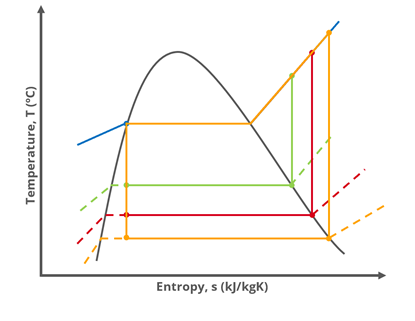
\includegraphics[width=9.5cm]{images/ts_diagram.png}
    \caption{T-s Diagram for Probable Design Evaporation Temperatures}
\end{figure}

\medskip
Using CoolProp [18], the team determined the performance parameters of the isolated heat pump cycle, namely, $Q_L$, $Q_H$, $W_{comp}$ and $COP$. With $W_{comp}$  or theoretical compressor work in mind, appropriate sizing for the compressor was determined. Next, code was developed which amalgamated the flat plate collector’s governing equations and, through iteration, allowed for the determination of the flat plate’s mean temperature. Figure 3.4 below depicts the complete iteration algorithm utilized in the MATLAB code.

\medskip
\begin{figure}[H]
    \centering
    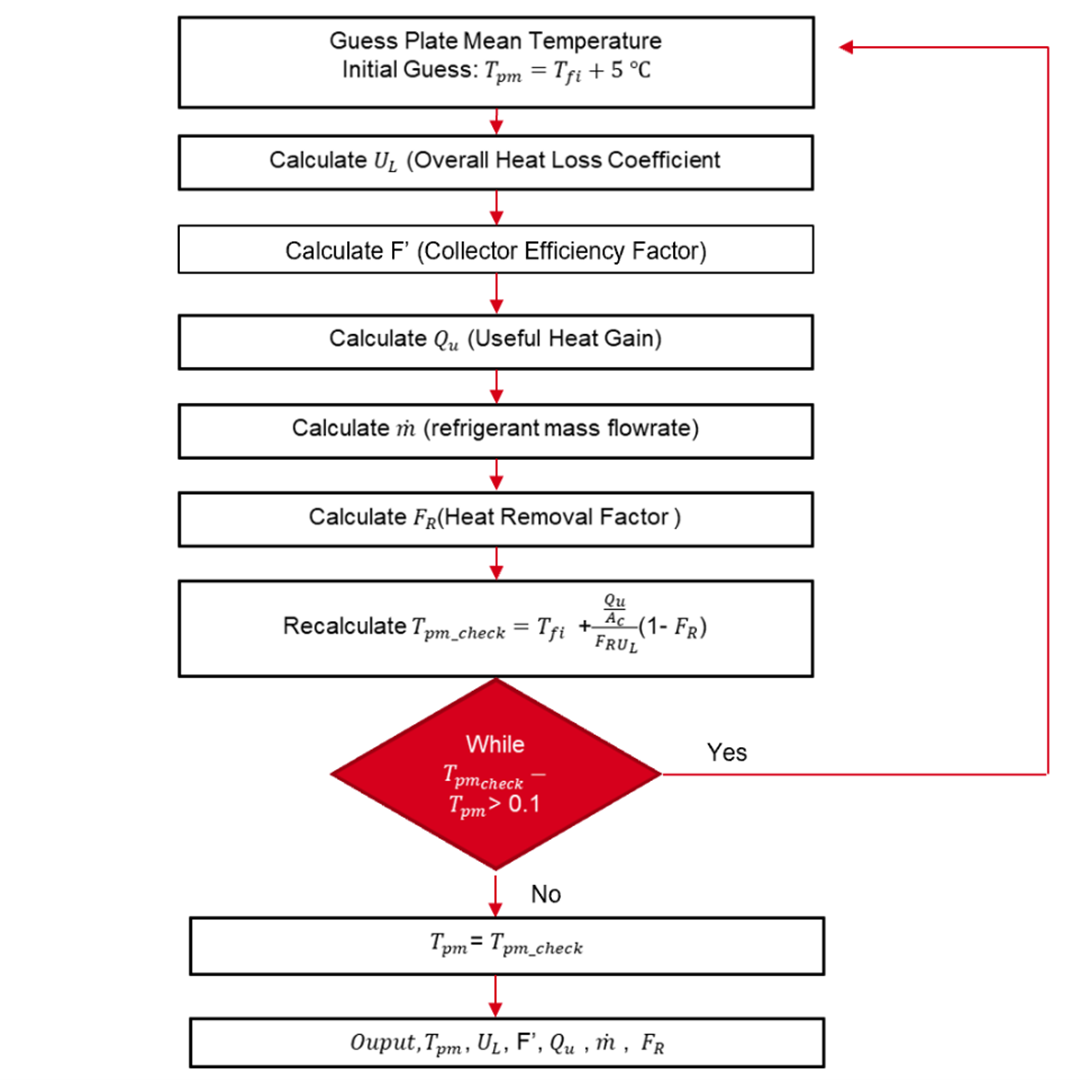
\includegraphics[width=12cm]{images/iterative_solution.png}
    \caption{Iterative Solution for Flat Plate Mean Temperature}
\end{figure}

\medskip
Once the flat plate’s mean temperature was determined, the collector’s useful heat gain, and, subsequently, the collector’s efficiency was evaluated for every data point in the evaporation temperature range. The evaporation temperature’s impact on the isolated heat pump cycle $COP$ is diametrically opposed to its impact on the useful heat gain of the collector: on one hand, the $COP$ of the heat pump cycle increases as the gap between the evaporation and condensation reservoir temperature is minimized, or when the chosen evaporation design temperature is elevated. On the other hand, the collector’s efficiency declines with the elevation of evaporation temperature as a result of increased heat losses from its surfaces. Noting this inverse relationship, it’s deducible that a plot of the product of $COP$ and Collector Efficiency (a quantity defined as the overall system $COP$) versus evaporation temperature would exhibit a characteristic inflection point at the evaporation temperature that maximizes both these inversely related parameters. For the DX-SAHP, the inflection point was seen to occur at -2\textdegree C. Knowing the design evaporation temperature, the team was able to subsequently determine the predicted collector efficiency, and the predicted useful, net collected heat. These values will later be leveraged to evaluate the theoretical performance of the DX-SAHP against the logged experimental performance. Using the code, the team also determined the system’s necessary flow rate, which supplemented the selection process of the remaining sub-components of the heat pump cycle.

\subsection{Insulation Selection}

Insulation is one of the most efficient ways to save energy by reducing heat loss during winter and thus lowering energy bills \cite{insulation}. Reducing heat loss in the collector means the compressor will have to do less work to meet the hot water requirements. For the flat plate collector, it was essential to investigate the concepts pertaining to location of any heat losses to the surroundings, type, thickness, and cost of insulation.

\medskip
In the solar flat plate collector, heat losses occur through the absorber plate by top losses. As the plate heats up, some of this heat is then transferred to R-134A (within the copper tubing of the collector that is bonded to the rear side of the aluminum absorber plate), while some of the heat is lost to the surroundings. The heat losses occurring through the back, and sides of the collector are respectively known as bottom and edge losses \cite{heat_losses}. From heat transfer and thermodynamic contexts, it is understood that these heat losses occur in the form of conduction, convection, and radiation as described in the sections above.\cite{heat_losses}.

\medskip
Based on the engineering analysis and design of the collector, the bottom and sides require insulation as to minimize any heat losses and the consideration of an insulation cover being required in case of probable exposure area that is responsible for the occurrence of any heat losses.

\medskip
The insulation materials representative of some of the materials commonly used in solar flat plate collectors and in the industry are as follows:

\medskip
\begin{itemize}[itemsep=3mm, parsep=-1mm]
    \item Fiberglass wool. 
    \item Rigid polyurethane foam.
    \item Mineral wool.
    \item Expanded polystyrene.
    \item Extruded polystyrene.
\end{itemize}

The following table represents the range of thermal conductivity values, temperature, and R-values \cite{thermal_insulation} for the mentioned types of insulation materials.

\medskip
\begin{table}[H]
\centering
\caption{Range for Thermal Conductivity, Temperature, and R-Value for Insulation}
\rowcolors{2}{gray!20}{white}
\begin{tabular}{|P{40mm}|P{35mm}|P{35mm}|P{35mm}|}
    \hline
    \rowcolor{orangeRed}
    Insulation Type & Thermal Conductivity, k $[W/mK]$ & Temperature Range & R Value [per inch of thickness] \\
    \hline
    Fiberglass Wool         & 0.023 - 0.040 & -195\textdegree C to 230\textdegree C & R-3.7 to R-4.2  \\
    Rigid Polyurethane Foam & 0.020 - 0.035 & 62\textdegree C to 93\textdegree C    & R-3.4 to R-6.7 \\
    Mineral Wool            & 0.033 - 0.040 & Maximum: 649\textdegree C             & R-3.7 to R-4.3 \\
    Expanded Polystyrene    & 0.030 - 0.040 & Maximum: 75\textdegree C              & R-3.9 to R-4.7 \\
    Extruded Polystyrene    & 0.025 - 0.040 & Maximum: 74\textdegree C              & R-5.0 to R-5.6 \\
    \hline
\end{tabular}
\end{table}

\medskip
The following table identifies the American Society for Testing and Materials (ASTM) specification, material type, and/or grade for some of the insulation materials that are commonly used in the industry \cite{insulation_design}.

\medskip
\begin{table}[H]
\centering
\caption{Common Types of Insulation - Based on ASTM}
\rowcolors{2}{gray!20}{white}
\begin{tabular}{|P{50mm}|P{50mm}|}
    \hline
    \rowcolor{orangeRed}
    Material & Insulation Standard \\
    \hline
    Cellular Glass   & ASTM C 552 Type II        \\
    Elastomeric      & ASTM C 534 Type I, Gr 1   \\
    Fiberglass       & ASTM C 547 Type I         \\
    Flexible Aerogel & ASTM C 1728 Type I, Gr 1B \\
    Phenolic         & ASTM C 1126 Type III      \\
    Polyethylene     & ASTM C 1427 Type I, Gr1   \\
    Polyisocyanurate & ASTM C 591 Type IV        \\
    Polystyrene      & ASTM C 578 Type XIII      \\
    \hline
\end{tabular}
\end{table}

\medskip
Based on the above analysis, mineral wool was selected as the insulating material to be used for the solar flat plate collector due to its excellent thermal properties. The mineral wool insulation was sponsored by Frank of FN Insulations. 

\medskip
Mineral wool has low thermal conductivity values, allowing for less heat to be passed through and lost to the surroundings. The suitable temperature range allows for use up to 649\textdegree C as this material will not melt until temperatures reach beyond 1,000\textdegree C. The R-values are within a range of R-3.7-R-4.3, allowing for it to suitably resist heat flow. In addition, mineral wool is naturally moisture resistant \cite{mineral_wool}.

\subsection{Glazing Selection}

Glazing refers to the top cover of the solar collector. It has three main purposes:

\medskip
\begin{enumerate}[itemsep=3mm, parsep=-1mm, label=\roman*.]
    \item Protect the internal components from the outside environment.
    \item Minimize heat loss due to convection and radiation from the absorber plate.
    \item Allow as much solar radiation through as possible.
\end{enumerate}

\medskip
The two main materials used for solar collector glazing are glass and polycarbonate.

\medskip
The main parameter that was considered when choosing the glazing is the transmittance. Transmissivity is a measure of how much light passes through the object for a given wavelength. For a solar collector, the glazing should let through as much sunlight as possible but be opaque to the infrared radiation emitted by the absorber plate. This will allow for the most heat gain possible. The secondary parameter, which should be minimized is the reflectance of the glazing. The reflectivity is represents the fraction of reflected solar rays. \cite{emissivity}.

\medskip
Another important factor to consider is the solar heat gain coefficient (SHGC). The SHGC is a measure of how much solar radiation is admitted. A high SHGC rating indicates that the materials are more effective at collecting solar heat, which is better for a solar collector \cite{epri}.

\medskip
\begin{table}[H]
\centering
\caption{Properties of Various Glazing Materials}
\rowcolors{2}{gray!20}{white}
\begin{tabular}{|P{31mm}|P{23mm}|P{23mm}|P{10mm}|P{34mm}|P{17mm}|}
    \hline
    \rowcolor{orangeRed}
    Glazing Type & Temperature Range & Transmissivity & SHGC \cite{glass_glazing}\cite{polycarbonate_glazing} & Thermal Expansion Coefficient $(in/in/F)$ & Density $(kg/m^3)$ \\
    \hline
    Low Iron Tempered Glass \cite{low_iron_glass}  & -50\textdegree C to 240\textdegree C & 91.5\% & $\sim 0.91$ & 4.9E-6  & 2530 \\
    Polycarbonate (Standard) \cite{polycarbonate} & -50\textdegree C to 120\textdegree C & 86\%   & $\sim 0.80$ & 3.75E-5 & 1197 \\
    Sun-Lite \cite{fiberglass}                 & -50\textdegree C to 120\textdegree C & 86\%   & $\sim 0.80$ & 3.6E-5  & 1200 \\
    Lexan 9034 \cite{lexan}               & -40\textdegree C to 100\textdegree C & 88\%   & $\sim 0.80$ & 3.75E-5 & 1197 \\
    SunTuf \cite{suntuf}                   & -40\textdegree C to 100\textdegree C & 90\%   & $\sim 0.80$ & 3.6E-5  & 1200 \\
    \hline
\end{tabular}
\end{table}

\medskip
As seen from Table 4 above, all the materials found met the temperature requirement of -30\textdegree C to 30\textdegree C. Low iron tempered glass was found to have the highest transmissivity, highest solar heat gain coefficient, and lowest coefficient of thermal expansion. Glass was found to be more opaque to the long wave radiation emitted by the absorber plate, and therefore better at trapping heat \cite{low_iron_glass_vs_regular}. Whereas polycarbonate was found to transmit more IR radiation \cite{plexiglass}. Additionally, polycarbonate will yellow over time from exposure to UV rays \cite{polycarbonate_yellowing}; this will reduce the amount of light transmitted by it. However, glass is more than two times heavier than the polycarbonate sheets and more prone to breaking. So extra care will need to be taken when installing it in the collector.

\subsection{Plate Material Selection}

The absorber plate is the component which absorbs solar radiation and emits it as infrared radiation. This heat is then absorbed by the copper piping and then the refrigerant. For this purpose, the plate must have high absorptivity, heat conductivity, and emissivity. The most common materials for the absorber plate are copper, aluminum, and steel; the thermal conductivities of these metals are $398 W/mK$, $247 W/mK$, and $45 W/mK$ respectively \cite{thermally_conductive_materials} \cite{thermal_conductivity_of_steel}. Steel was found to have too low thermal conductivity for this application. The price of copper was \$9.55/kg \cite{copper_prices} and aluminum was \$6.33/kg \cite{aluminum_prices}. Aluminum was selected for our application because it was more readily available.

\medskip
A selective coating was applied to the absorber plate to increase the amount of sunlight absorbed.Thurmalox 250 was identified as a coating specifically suited for solar thermal collector application. The coating possesses a high absorbance and low emissivity, so all the absorbed heat will be transferred to the aluminum plate. It is capable of withstanding high temperatures and is  UV resistant. \cite{high_temp_coating}.

\subsection{Manifold Design}

To determine the copper tube design beneath the absorber plate of the solar flat plate collector, it was convenient to create a two-dimensional drawing to determine the layout. The design of the tubing helped determine the overall length of tubing that would be required. A serpentine tube design was selected as it maximizes the amount of surface area, and for R-134A, for heat transfer to occur within a limited amount of space \cite{serpentine_bending}.

\medskip
The serpentine copper tube design for the flat plate collector was completed based upon the following criteria:

\medskip
\begin{enumerate}[itemsep=3mm, parsep=-1mm, label=\roman*.]
    \item Tube pitch of 3/4 inches [19.05 mm].
    \item Tube bend diameter of 3 15/16” [100 mm].
    \item Leave 1 15/16” [50mm] on each side of absorber plate.
\end{enumerate}

\medskip
In the following figure, two designs were created, (a) and (b). Both designs have an equal manifold spacing. The design for (a) was selected as this design leads to a greater surface area allowing for more heat transfer to occur. With the design for (a) having more U-bends in the tubes, this allows for more time for heat transfer to take place with R-134A. 

\begin{figure}[ht]
    \centering
    \subfloat[\centering Horizontally Spaced Manifold] {{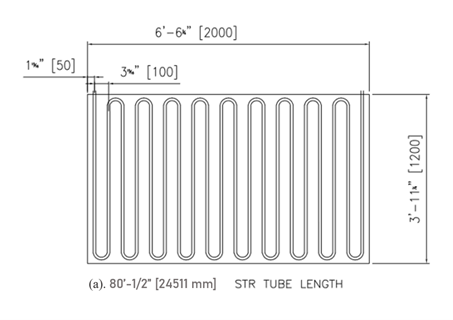
\includegraphics[width=7.7cm]{images/manifold_type_a.png}}}
    \qquad
    \subfloat[\centering Vertically Spaced Manifold] {{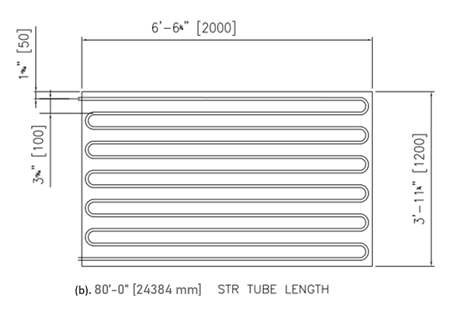
\includegraphics[width=7.7cm]{images/manifold_type_b.png}}}
    \caption{Two-Dimensional Designs of Serpentine Copper Tube Manifold}
\end{figure}

\subsection{Final Collector Model}

\begin{figure}[H]
    \centering
    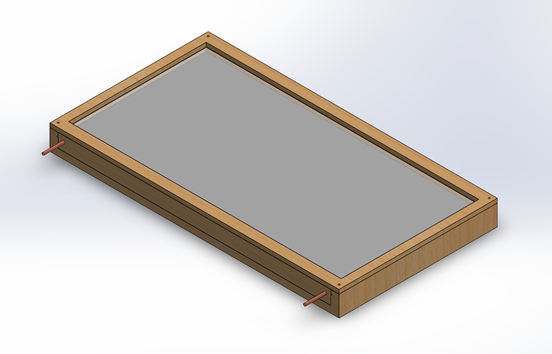
\includegraphics[width=\textwidth]{images/collector_assembly.png}
    \caption{SOLIDWORKS Assembly of Solar Thermal Collector}
\end{figure}


\medskip
Although the collector frame is a simple enclosure, sizing limits and assembly considerations has to be considered. The wood casing was created in multiple parts and grooves were added to account for the thermal expansions of both the glass and absorber plates during winter thermal contractions and summer thermal expansions. 

\medskip
The depth of the grooves were determined using the equation for linear thermal expansion.
\begin{align}
    \Delta L = \alpha_L L_c \Delta T
\end{align}

\medskip
The order in which the components were assembled was taken in consideration to avoid scenarios where components are blocked by other ones. As component selection was finalized, fitment tolerances were added.
\medskip

\section{Component Selection}

For component matching, external to the solar flat plate collector, suitable components and materials for the system based on data and design parameters were selected. The components included the compressor, condenser, expansion valve, control system, and minor parts. The evaluation of manufacturing methods and metal-joining processes, such as, brazing, soldering and/or welding, and use of items such as couplings, and tube adapters were also considered.

\subsection{Compressor Selection}

A compressor is required after the collector to meet the domestic hot water requirements.

\medskip
The compressor selection was based on the lowest evaporating temperature of -6°C. However, the operating envelope of the compressor can reach an evaporation temperature of -8\textdegree C before it automatically shuts down. The fixed speed scroll compressor will allow for the domestic hot water to be heated to 55\textdegree C. The following figure shows the operating envelope of the compressor sponsored by Emerson.

\begin{figure}[H]
    \centering
    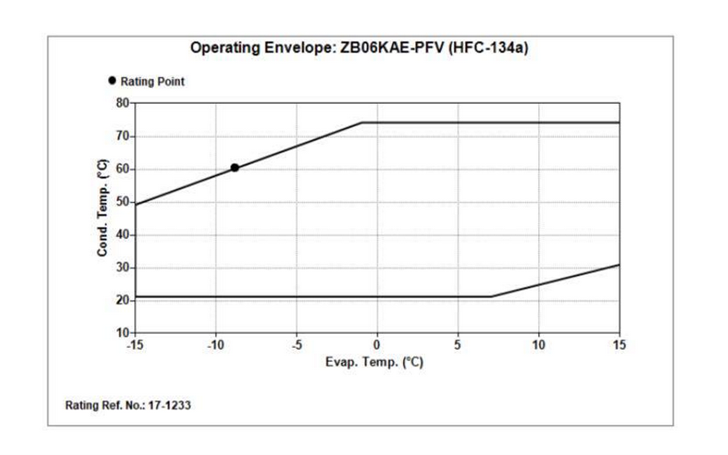
\includegraphics[width=8cm]{images/operating_envelope.png}
    \caption{Operating Envelope of the Fixed Speed Scroll Compressor}
\end{figure}

\medskip
The compressor was also evaluated based on the criteria shown below: 

\medskip
\begin{enumerate}[itemsep=3mm, parsep=-1mm, label=\roman*.]
    \item Compatibility with R-134A.
    \item Evaporation Temperature Range: -6\textdegree C to 14\textdegree C.
    \item Compressor Rated Power: 0.75 HP to 1.25 HP.
\end{enumerate}

\medskip
The power requirement for the compressor was found to be 1.138 horsepower based on the required flow rate. The single-phase, 208/230 Volts at 60 Hertz, fixed speed scroll compressor was selected for this project. These types are commonly used for many residential heat pump applications. It may be applied for the purposes of the DX-SAHP as it operates at low capacities, requiring less input power. Compared to its hermetic reciprocating counterparts, the Copeland scroll compressor is simpler to incorporate into new designs and additional design costs \cite{copeland}. The benefits of this type were previously discussed under the HVAC Types in this report.

\medskip
The following figure shows the fixed speed scroll compressor.

\medskip
\begin{figure}[H]
    \centering
    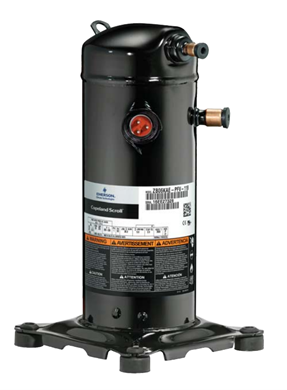
\includegraphics[width=4.5cm]{images/fixed_speed_compressor.png}
    \caption{Fixed Speed Scroll Compressor}
\end{figure}

\medskip
The compatibility between the fixed speed scroll compressor and electronic expansion valve is crucial as this controls the pressure differential of R-134A through the compressor and the amount of flow rate through the valve. The external sponsors of Emerson were provided with the design specifications, controller requirements, and refrigerant parameters to size these components. The copper piping, having a diameter of 3/8 inches, is to be connected to the suction and discharge of the compressor and valve. The determination of the diameters and materials of these lines were communicated with the sponsor as to allow the easiest route for metal-joining and installation purposes. The external piping to the suction/discharge lines of both the compressor and valve, were accomplished by brazing the copper piping to the connecting tubes and additional pipe connections and fittings were used. 

\subsection{Condenser Selection}

A series of condenser designs were considered before settling on the final configuration. However, all the designs had to meet the five basic criteria below:

\medskip
\begin{enumerate}[itemsep=3mm, parsep=-1mm, label=\roman*.]
    \item Maximum condensing coil temperature of 85\textdegree C.
    \item Maximum condensing coil pressure of 3800kPa.
    \item Total possible heat rejection of 2.5kW.
    \item Condensing coil must be compatible with R-134A.
    \item Storage capacity of 225L.
\end{enumerate}

\medskip
The initial idea for the condenser was to use an insulated water tank with an integrated helical copper coil on the inside shown in Figure 3.10 below. However, sourcing these pre-built tanks with the aforementioned criteria was difficult. This condensing unit was broken down into its basic components in the next designs.

\medskip
\begin{figure}[H]
    \centering
    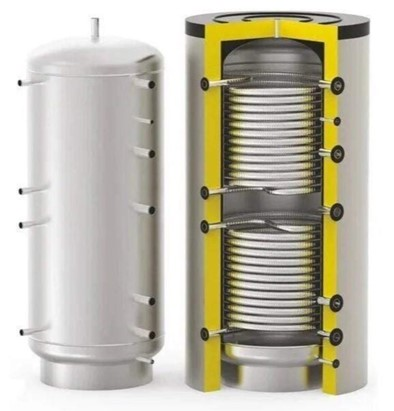
\includegraphics[width=5 cm]{images/water_tank_condenser.jpg}
    \caption{Water Tank with Two Condensing Coils \cite{water_tank_selection}}
\end{figure}

\medskip
The second design consisted of an insulated water tank with an external heat exchanger as shown in Figure 3.11 below. The water would be pumped from a cold-water storage tank, through the now external heat exchanger, and stored in an insulated tank. The external heat exchanger shown is a coaxial coil condenser. This configuration required the use of a pressure actuated water regulating valve to control the flow rate of water into the coaxial condenser coil. The valve opening is controlled by the pressure in the refrigerant side. This was to allow the water to be heated from 10\textdegree C to 55\textdegree C in a single pass through the coil. There were two main drawbacks to this design. The first being that, since the water is continually being heated from 10\textdegree C to 55\textdegree C, the compressor would constantly be working at its maximum capacity; this in turn would increase the work in $W_in$ and thus reduce the $COP$. Secondly, if the water is not heated to 55\textdegree C in a single pass, there is no process to reuse and reheat this water. This may lead to frequently wasting water during testing as the unheated water would have to be disposed. Therefore, the system was reworked.

\medskip
\begin{figure}[H]
    \centering
    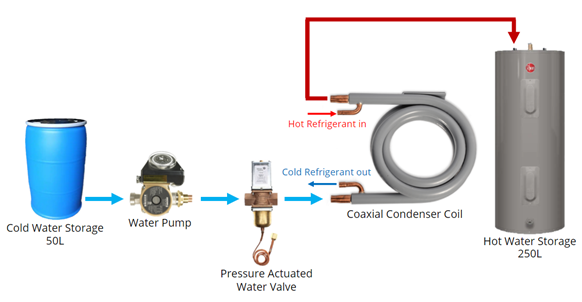
\includegraphics[width=12cm]{images/condensor2.png}
    \caption{Second Condensing Design}
\end{figure}

\medskip
The third iteration of the design, shown in Figure 3.12 below, consisted of a water recirculation system to address the previous problems. Additionally, the use of a cold-water storage tank was not required with this design. The main disadvantage of this design is that, as the water heats up, the rate of heat transfer between the refrigerant and water will decrease leading to a lower $COP$. However, as the water temperature difference decreases, the compressor draws less power to heat the preheated water. This means that the overall $COP$ of the system would be higher than if there was no recirculation. Furthermore, since the water is recirculated, the use of a pressure actuated valve is no longer required. The valve may cause a decrease in $COP$ due to the compressor doing more work to heat the water from 10\textdegree C to 55\textdegree C during startup even if sunlight is not available. In a recirculation system without the pressure actuated valve, the water will most efficiently be heated when there is available sunlight and will not have to rely on the compressor during periods of low irradiance.

\medskip
\begin{figure}[H]
    \centering
    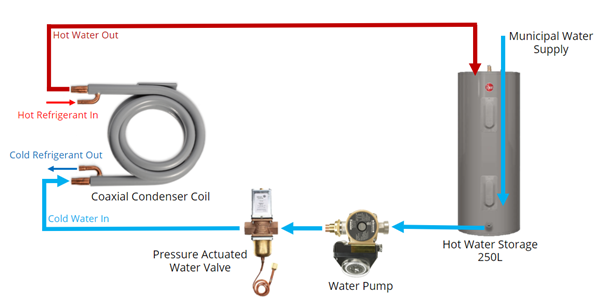
\includegraphics[width=12cm]{images/condensor3.png}
    \caption{Third Condensing Design}
\end{figure}

\medskip
This results in the fourth and final design, without the pressure actuated water regulating valve, shown in Figure 3.13 below. The water is recirculated from the hot-water storage tank to the condenser coil and back by the pump.

\medskip
\begin{figure}[H]
    \centering
    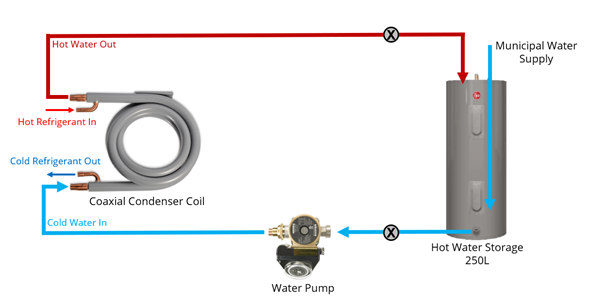
\includegraphics[width=12cm]{images/condensor4.png}
    \caption{Fourth (Final) Condensing Design}
\end{figure}

\medskip
For this final design, the components were selected as shown below.

\subsubsection{Condenser Piping}

\medskip
Sharkbite connections with \nicefrac{3}{4}" PEX piping was chosen for ease of assembly. The allowable temperature range was also 0.5\textdegree C to 93.3\textdegree C \cite{pex_tech}, more than enough for this application. 

\subsubsection{Hot-Water Tank}

\medskip
A 250L hot-water tank could not be easily sourced, so for the purpose of testing, a 178L Rheem hot-water tank was chosen \cite{hot_water_tank}. Once the 178L is heated to 55\textdegree C, the water can be dumped to allow for new water to be heated.

\medskip
\begin{figure}[H]
    \centering
    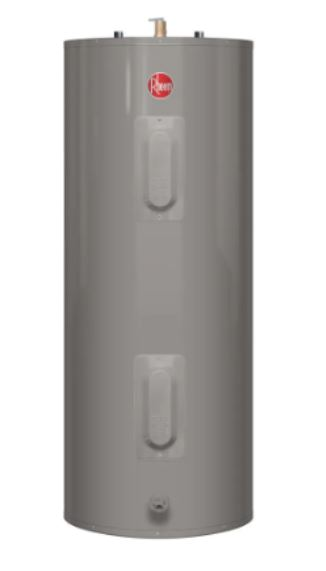
\includegraphics[width=3.5cm]{images/rheem_178L_tank.JPG}
    \caption{Rheem 178L Hot-Water Tank}
\end{figure}

\subsubsection{Condenser Coil}

\medskip
The external heat exchanger is a \nicefrac{3}{4} ton counterflow coaxial coil condenser \cite{coax_coil}.

\medskip
\begin{figure}[H]
    \centering
    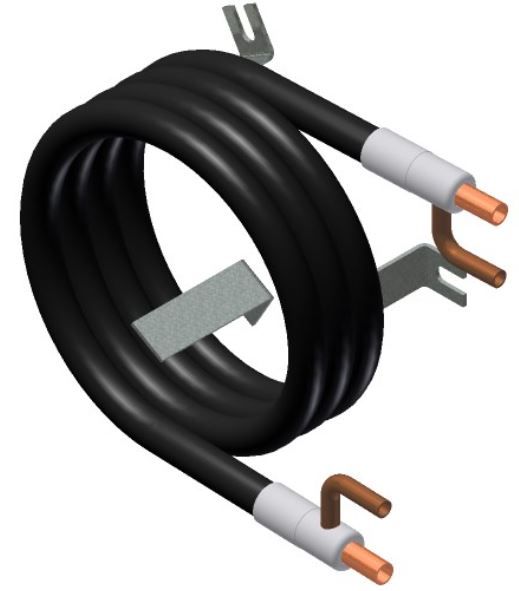
\includegraphics[width=4cm]{images/coax_coil.JPG}
    \caption{\nicefrac{3}{4} ton counter flow coax coil}
\end{figure}

\subsubsection{Water Side Pressure Drop}

\medskip
The pressure drop had to be found to find a suitable water pump. The sources of the drop in pressure are from pipe friction, change in height, pipe bends, and the condenser coil itself. These were calculated for a \nicefrac{3}{4}” pipe as shown below:

The pressure drop due to friction can be found for PEX piping from the tables shown in Figure 3.16 below.

\begin{figure}[H]
    \centering
    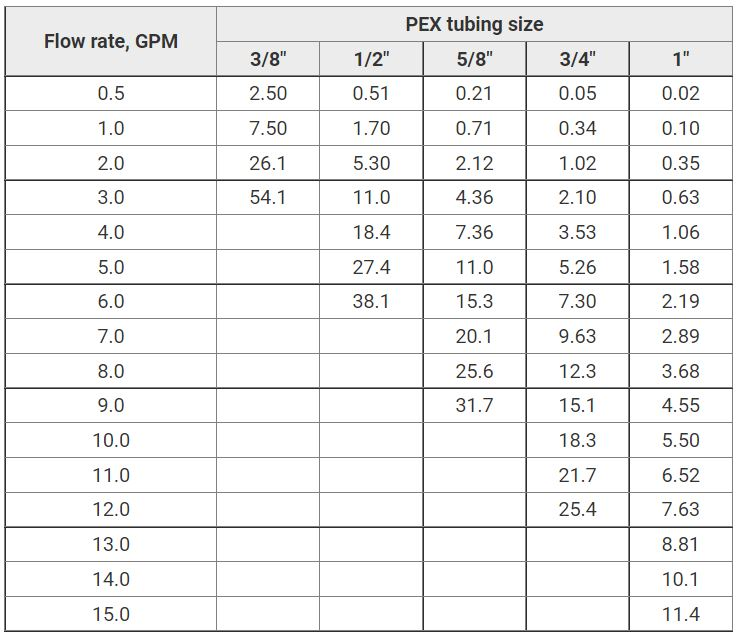
\includegraphics[width=8.5cm]{images/pex_pressure_drop.JPG}
    \caption{PEX Piping Pressure Drop Table}
\end{figure}

\medskip
The required flow rate can be calculated from the following \cite{water_valve}:
\begin{align}
    Flow\ [GPM] = \ddfrac{Tons\ of\ Refrigeration \times 15000}{500\times (T_{out}-T_{in})}
\end{align}

\medskip
This tells us the required flow rate to heat the water from the inlet to the outlet temperature (10 \textdegree C to 55 \textdegree C), in a single pass through the condenser, is 0.5GPM. However, since this design recirculates the water, it is not required to go from 10 \textdegree C to 55 \textdegree C in a single pass. This means that for faster flow rates, the change in water temperature would decrease, and more passes through the condenser are needed. For a flow rate of 1.8GPM, the change in temperature is 12.5 \textdegree C.

\medskip
The pressure drop from a change in height is calculated as \cite{fluid_mechanics}:
\begin{align}
    P_h = \rho g h
\end{align}

\medskip
The change in height will depend on the height of the piping above the hot water tank since it is being recirculated.

\medskip
The pressure drop from the coaxial condenser coil can be found from the manufacture specified table shown in Figure 3.17 below:

\begin{figure}[H]
    \centering
    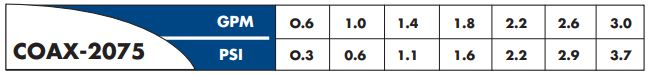
\includegraphics[width=10cm]{images/coax_coil_pressure_drop.JPG}
    \caption{Coaxial Coil Pressure Drop Table}
\end{figure}

\medskip
Finally, the pressure drop due to bends in the piping can be calculated as \cite{fluid_mechanics}:
\begin{align}
    \Delta P_{elbow} = \ddfrac{K_L\rho w}{2}
\end{align}

\medskip
$K_L$ is the loss coefficient of the specified component or elbow. The loss coefficient for a regular 90\textdegree threaded elbow is 1.5.

\subsubsection{Hot Water Recirculating Pump}

Since the water is recirculating, the pump must meet the minimum required head which was found to be $\sim4.5ft$ for a flow rate of 2GPM making conservative estimates for the length of piping, number of elbows, change in height, and pressure drop from the condenser.

\medskip
The Astro Express 2 hot water pump \cite{astro_express} was selected for this purpose. It can handle temperatures up to 60\textdegree C. The pump curves are shown in Figure 3.18 below.

\begin{figure}[H]
    \centering
    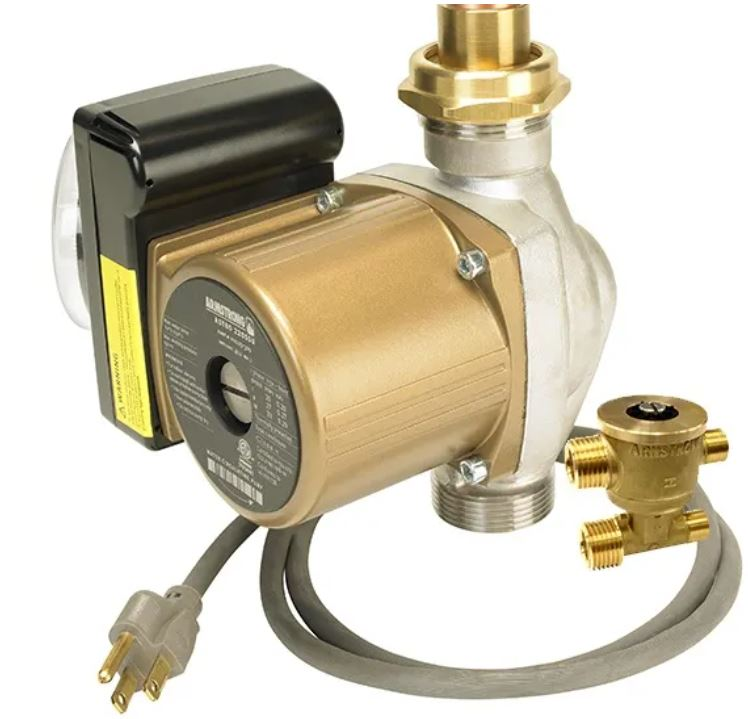
\includegraphics[width=2.5cm]{images/astro_express.JPG}
    \caption{Astro Express 2 hot water recirculating pump}
\end{figure}

\begin{figure}[H]
    \centering
    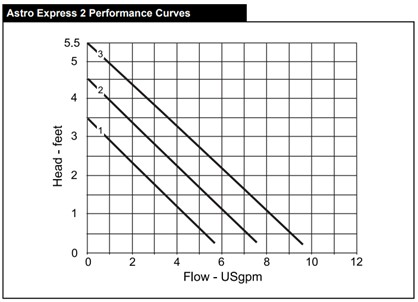
\includegraphics[width=10cm]{images/astro_express_performance.jpg}
    \caption{Astro Express 2 Pump Curves}
\end{figure}

\subsection{Electronic Expansion Valve Selection}

Selection of electronic expansion valves (EXV) was based on the following criteria:

\medskip
\begin{enumerate}[itemsep=3mm, parsep=-1mm, label=\roman*.]
    \item Suitable for HFC refrigerants (i.e., R-134A).
    \item Rated Capacity (kW).
\end{enumerate}

\medskip
Firstly, the selected valve must be compatible with the chosen refrigerant (i.e., R-134A).

\medskip
Secondly, the expansion valve must be able to provide the needed pressure reduction for system parameters. This is usually given by a vendor through an EXV’s capacity rating, which references the system’s heat removal rate in kW. Vendors provide a capacity rating for the following refrigerant conditions, based on AHRI standards \cite{exv_performance}:

\medskip
\begin{table}[H]
\centering
\caption{AHRI Standard Rating Conditions for EXV}
\rowcolors{2}{gray!20}{white}
\begin{tabular}{|P{27mm}|P{35mm}|P{40mm}|P{40mm}|}
    \hline
    \rowcolor{orangeRed}
    Standard Rating Condition & Liquid Temperature at EXV Inlet & Condensing Temperature at EXV Inlet & Evaporating Temperature at EXV Outlet \\
    \hline
    A & 37\textdegree C & 38\textdegree C & 4\textdegree C \\
    \hline
\end{tabular}
\end{table}

\medskip
If the above standard is not used, vendors must specify the operating conditions used instead for their stated rating.

\medskip
Since these operating conditions differ from the ones in the DX-SAHP, a correction factor must be added to the required capacity rating, to compare it with ratings from the vendor. The following information was needed to determine the correction factor:

\medskip
\begin{enumerate}[itemsep=3mm, parsep=-1mm, label=\roman*.]
	\item Refrigerant: R-134A.
	\item Condenser capacity: $Q_L = 2.5 kW$.
	\item Evaporating temperature: $T_{evap} = \SI{-10}{\celsius}$.
	\item Condenser temperature: $T_{cond} = \SI{60}{\celsius}$.
	\item Subcooling: Assume subcooling of $\Delta T_{sub} = 4K$ at inlet of EXV.
\end{enumerate}

\medskip
Based on these conditions, the team received help from Emerson, one of the project sponsors, in selecting the electronic expansion valve. The EX2 3/8X1/2 ODF expansion valve from Emerson was chosen, and Emerson kindly provided the product as well.
\medskip

\subsection{Refrigerant Piping}

Piping is an essential part of a heat pump; it carries the energy gained by the collector and compressor to be released in the condenser. A preliminary analysis was done to determine the drop in pressure between major components in the system. This pressure drop was considered to be from friction in the pipe, elbows, and changes in height. The total pressure drop of the system was necessary in determining the compressor size. The variable definitions for all the equations below can be found in Appendix A.

\medskip
The equation for pressure drop due to friction in a circular pipe is given as \cite{fluid_mechanics}:
\begin{align}
    \Delta P_f = \ddfrac{fL_p \rho w^2}{2D_i}
\end{align}

\medskip
The friction factor, f, was calculated separately for laminar and turbulent flows; however, in this system, only turbulent flows were found. For turbulent flow, the Colebrook White equation \cite{fluid_mechanics} was used to calculate the friction factor. This was solved by moving all terms to one side and using the \verb|fzero| MATLAB \cite{MATLAB} function to iteratively solve for the friction factor.
\begin{align}
    \frac{1}{\sqrt{f}} = -2.0log\left( \ddfrac{\frac{e}{D_i}}{3.7} + \frac{2.51}{Re\sqrt{f}}\right) 
\end{align}

The Reynold’s number determines the type of flow (i.e., Laminar, turbulent, or transitioning). If greater than 2320, the flow was considered turbulent. The Reynold’s Number was calculated as \cite{fluid_mechanics}:
\begin{align}
    Re = \ddfrac{wD_i}{\nu} = \ddfrac{\rho w D_i}{\mu}
\end{align}

\medskip
The values of density and viscosity were found using MATLAB to access CoolProp [18]. By specifying two state parameters, temperature and quality, the density and viscosity were obtained.

\medskip
The velocity of the refrigerant was calculated as:
\begin{align}
    w = \ddfrac{\dot m}{\frac{\rho \pi D_i^2}{4}}
\end{align}

\medskip
The pipe length between sections was assumed to be one meter for these calculations. Therefore, the pressure drop is shown per meter.

\medskip
The pressure drops were found for each section as described below:

\medskip
\begin{enumerate}[itemsep=3mm, parsep=-1mm, label= S\arabic*:]
	\item Between 1 (Compressor) and 2 (Condenser Inlet).
    \item Between 2 (Condenser Exit) and 3 (Expansion Valve).
    \item Between 3 (Expansion valve) and 4 (Evaporator Inlet).
    \item Between 4 (Evaporator Exit) and 1 (Compressor).
\end{enumerate}

\begin{figure}[H]
    \centering
    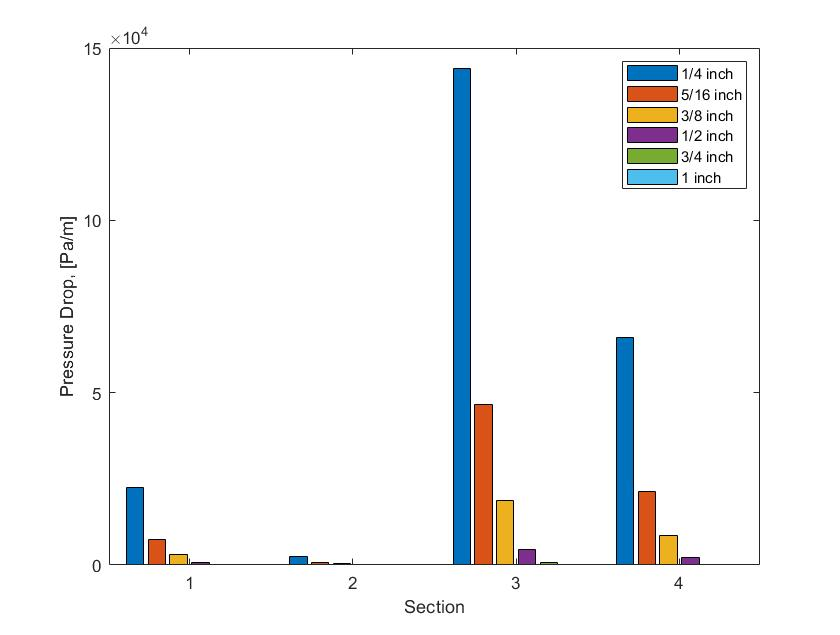
\includegraphics[width=11cm]{images/friction_pressure_drop.jpg}
    \caption{Pressure Drop for \nicefrac{1}{4}, \nicefrac{5}{16}, \nicefrac{3}{8}, \nicefrac{1}{2}, \nicefrac{3}{4}, and 1 inch Diameter Piping at each Section}
\end{figure}

\medskip
As seen from Figures 3.10 \& 3.11 above, as the diameter of the piping decreased, the pressure drop per meter increased drastically. Based on these values however, the pressure drop due to friction for diameters greater than \nicefrac{1}{4}” is insignificant considering the system operating pressures that range from $750kPa$ to $3800kPa$. Additionally, the piping for these sections are all less than a meter.

\medskip
The pressure drop due to elbows was calculated as follows \cite{fluid_mechanics}:
\begin{align}
    \Delta P_e = \ddfrac{K_L \rho w^2}{2}
\end{align}

\medskip
$K_L$ is the loss coefficient of the specified component or elbow. The loss coefficient for a long radius 90\textdegree \ flanged elbow is 0.2 and the loss coefficient for a regular 90\textdegree \ threaded elbow is 1.5 \cite{fluid_mechanics}.

\medskip
The pressure drop due to a change in height was calculated as \cite{fluid_mechanics}:
\begin{align}
    \Delta P = \rho g \Delta z
\end{align}

\medskip
The pressure drop due to elbows are shown for one elbow for each section below.

\medskip
\begin{figure}[H]
    \centering
    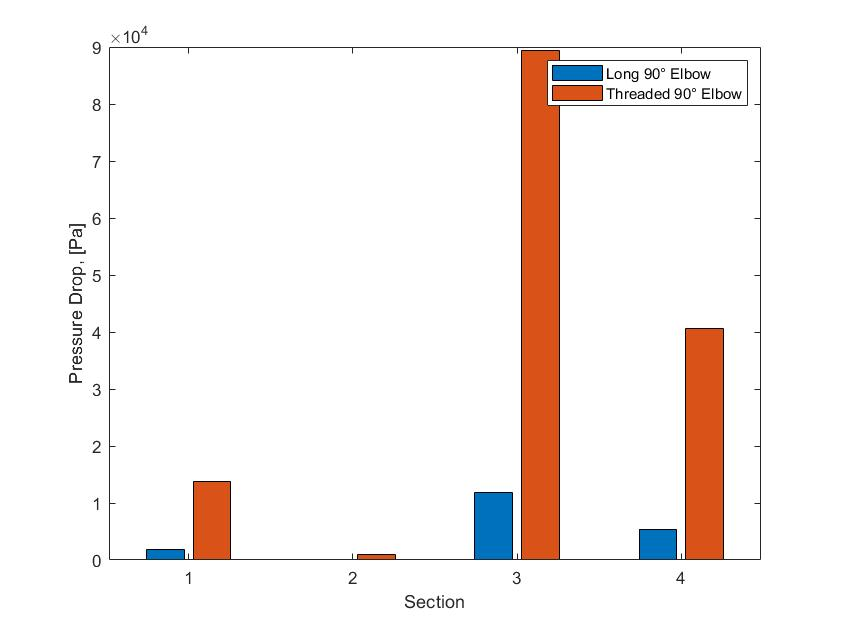
\includegraphics[width=11cm]{images/1-4in_Elbow Pressure_Drop.jpg}
    \caption{Pressure Drop from a Long Radius 90\textdegree \ Elbow vs. a Threaded 90\textdegree \ Elbow for a \nicefrac{1}{4} inch Pipe}
\end{figure}
\begin{figure}[H]
    \centering
    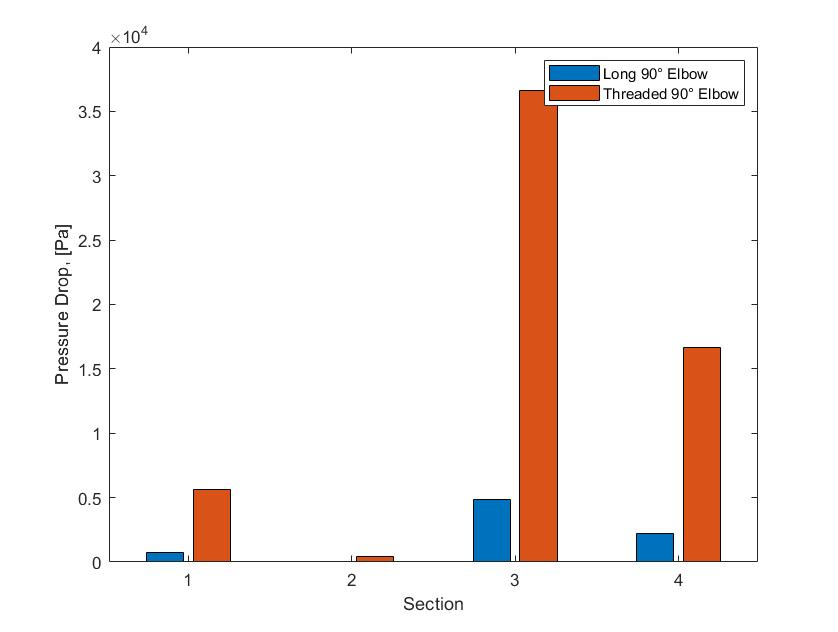
\includegraphics[width=11cm]{images/5-16in_Elbow Pressure_Drop.jpg}
    \caption{Pressure Drop from a Long Radius 90\textdegree \ Elbow vs. a Threaded 90\textdegree \ Elbow for a \nicefrac{5}{16} inch Pipe}
\end{figure}
\begin{figure}[H]
    \centering
    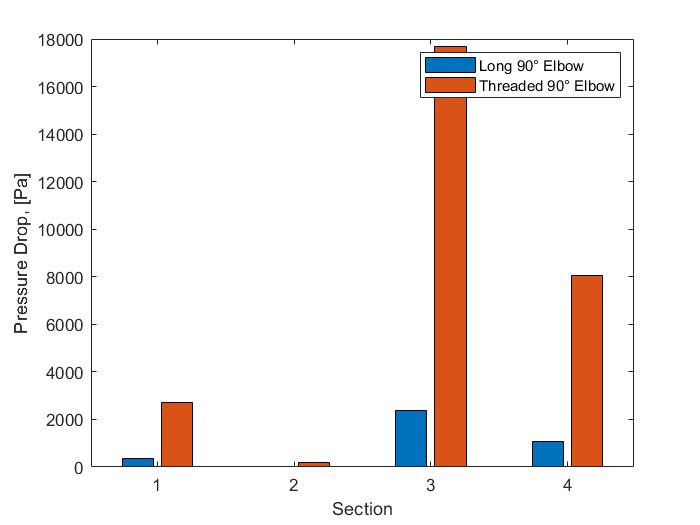
\includegraphics[width=11cm]{images/3-8in_Elbow Pressure_Drop.jpg}
    \caption{Pressure Drop from a Long Radius 90\textdegree \ Elbow vs. a Threaded 90\textdegree \ Elbow for a \nicefrac{3}{8} inch Pipe}
\end{figure}
\begin{figure}[H]
    \centering
    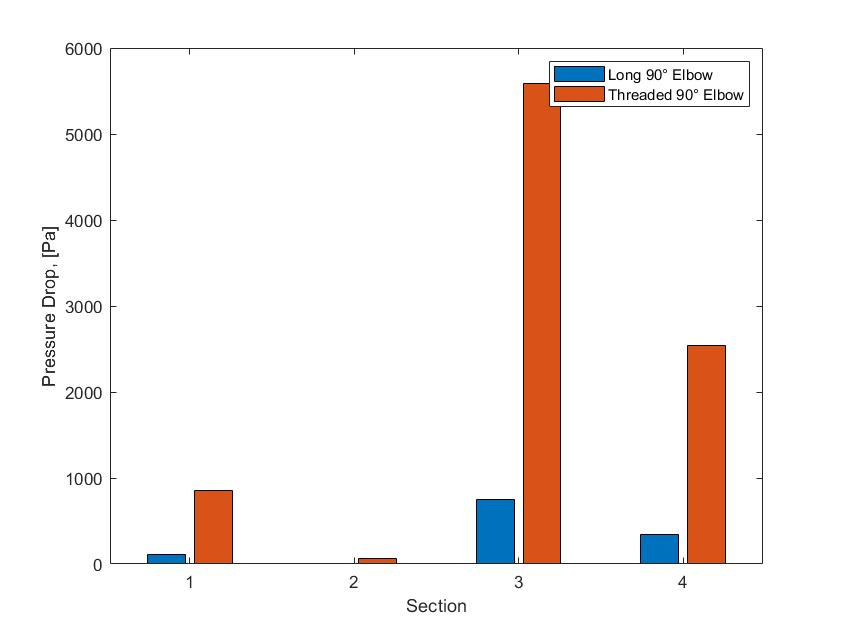
\includegraphics[width=11cm]{images/1-2in_Elbow Pressure_Drop.jpg}
    \caption{Pressure Drop from a Long Radius 90\textdegree \ Elbow vs. a Threaded 90\textdegree \ Elbow for a \nicefrac{1}{2} inch Pipe}
\end{figure}
\begin{figure}[H]
    \centering
    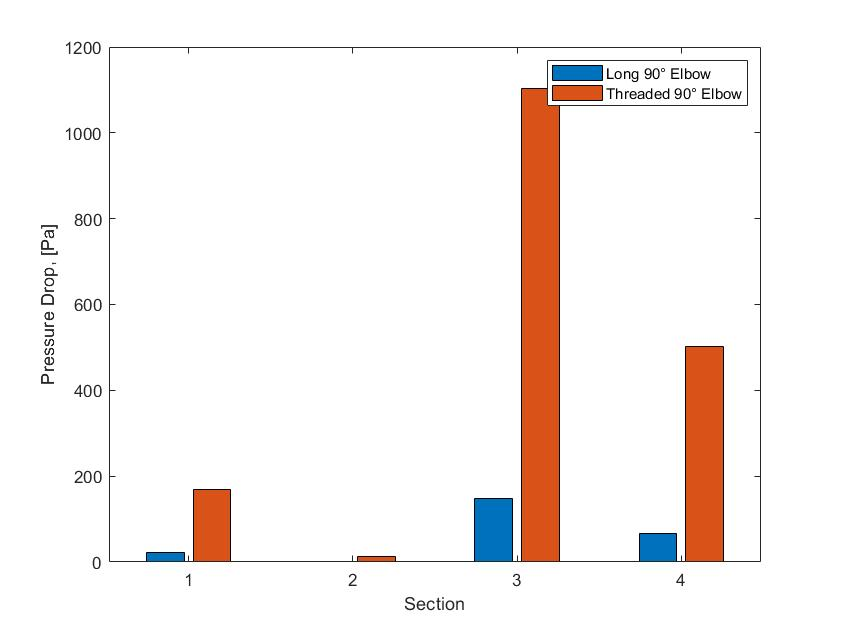
\includegraphics[width=11cm]{images/3-4in_Elbow Pressure_Drop.jpg}
    \caption{Pressure Drop from a Long Radius 90\textdegree \ Elbow vs. a Threaded 90\textdegree \ Elbow for a \nicefrac{3}{4} inch Pipe}
\end{figure}
\begin{figure}[H]
    \centering
    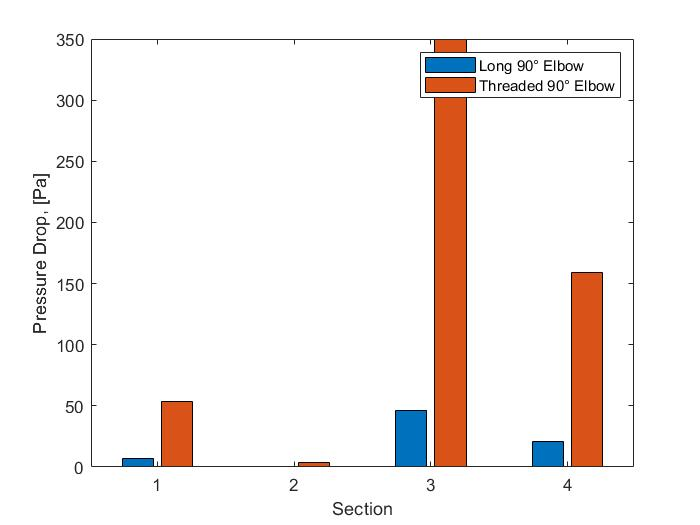
\includegraphics[width=11cm]{images/1in_Elbow Pressure_Drop.jpg}
    \caption{Pressure Drop from a Long Radius 90\textdegree \ Elbow vs. a Threaded 90\textdegree \ Elbow for a 1 inch Pipe}
\end{figure}

\medskip
As seen from Figures 3.20 - 3.26 above, the drop in pressure follows the same trend when decreasing the pipe diameter; smaller diameter has larger pressure drops. Additionally, the threaded 90\textdegree \ elbow yields more drop in pressure than the pipe with a large radius elbow as expected.

\medskip
When considering the operating point of the entire system from $750kPa$ – $3800kPa$, the pressure drops due to the piping is insignificant. The currently built refrigerant side piping uses \nicefrac{5}{16} and \nicefrac{3}{8} inch pipes. The maximum pressure drop was found to occur between 3 (Expansion valve) and 4 (Evaporator Inlet). The piping length between these sections in the design is less than 0.5m. In this section, the maximum pressure drop from friction for \nicefrac{5}{16} inch piping was found to be $46.5kPa$ per meter. The maximum pressure drop from elbows for \nicefrac{5}{16} was found to be $36.6kPa$ per elbow. The maximum pressure drop from friction for \nicefrac{3}{8} inch piping was found to be $18.6kPa$ per meter. The maximum pressure drop from elbows for \nicefrac{3}{8} was found to be $17.7kPa$ per elbow. Due to the compact system design, the pressure drop due to piping can be considered to be negligible.

\subsection{Accessory Parts}

\subsubsection{Receiver}

A receiver was added as per recommendations from Emerson and the HVAC contractor from Chinook Refrigeration. The receiver goes after the condensing unit and before the electronic expansion valve. It stores any excess refrigerant that is not being circulated around the system. Since the DX-SAHP system will be operating through a wide range of ambient conditions, there will be several mass flow rates implemented, and thus a need exists for a method to store the excess refrigerant. Having the receiver ensures space in the system to store the excess refrigerant - preventing it from pooling elsewhere.

\medskip
\begin{figure}[H]
    \centering
    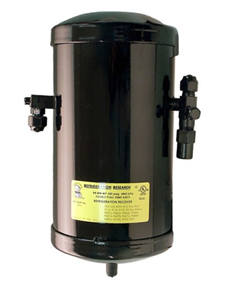
\includegraphics[width=3.5cm]{images/reciever.png}
    \caption{Refrigeration Research 3 lb. Receiver}
\end{figure}

\medskip
A Refrigeration Research 3 lb 1/4" SAE X 1/4" SAE Vertical Receiver \cite{receiver} was selected due to its availability for easy pick-up in Calgary, and an adequate refrigerant storing capacity of 3 lbs. This capacity was chosen with recommendations from the team’s contact at Emerson. 

\subsubsection{Filter Drier}

To keep the system working at optimal conditions, it is necessary to ensure that there are as little contaminants as possible. The potential contaminants in this system are water, copper shavings, or other contaminants during installation. The filter drier ensures these contaminants are not circulated throughout the system and causing damage; it is installed in the liquid-line of the heat pump before the sight glass \cite{sight_glass}.

\medskip
\begin{figure}[H]
    \centering
    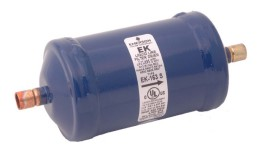
\includegraphics[width=3.5cm]{images/filter_drier.jpg}
    \caption{EK083S Filter Drier \cite{filter_drier}}
\end{figure}

\subsubsection{Sight Glass}

The sight glass is needed to view the level of the refrigerant to ensure proper operation. If there are bubbles seen through the sight glass it indicates that there is not enough refrigerant in the system. Additionally, the refrigerant must be subcooled before entering the EXV; therefore, the sight glass is installed before the EXV to ensure only liquid enters it \cite{sight_glass_install}.

\medskip
\begin{figure}[H]
    \centering
    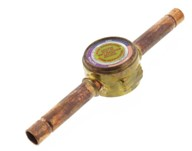
\includegraphics[width=3.5cm]{images/sight_glass.jpg}
    \caption{\nicefrac{3}{8}" ODF HMI-1TT3 Hermetic Sight Glass Moisture Indicator \cite{liquid_sight_glass}}
\end{figure}

\section{Control System}

The philosophy of having a control system for this design lies in the fact that the heat pump needs to adapt to varying ambient conditions to still meet the desired heat load. For instance, when there is less available sunlight, the refrigerant mass flow rate must be lowered, so the refrigerant can spend an adequate amount of time in the solar thermal collector and fully evaporate.

\subsection{Mass Flow Rate Control}

The mass flow rate of the refrigerant is an important control parameter and dictates how fast the refrigerant is flowing through the system. It is critical that the refrigerant enters the compressor as at least a saturated vapor, as any liquid-vapor mixture will damage the compressor. The refrigerant must spend enough time in the solar collector to ensure full phase-change is achieved. The time spent in the collector is directly linked to mass flow rate and thus it is critical that this parameter be controlled. For example, during colder conditions where there is less available sunlight, the system needs to be able to lower the flow rate so that the refrigerant can spend more time in the collector to completely changing phase.

\medskip
Mass flow rate will be controlled by the electronic expansion valve. There is a stepper motor in the valve that incrementally opens and closes the valve opening, to adjust the flow rate. This stepper motor responds to electronic signals that will be fed by an external controller. The Emerson super heat controller (Model: XEV12D) was selected as it is compatible with the system’s chosen electronic expansion valve. This superheat controller was generously provided by the team’s industry sponsor, Emerson. The controller input parameters include the refrigerant type, and the solar collector exit temperature and pressure. The temperature and pressure measurements will be given by an 20J NTC thermistor temperature sensor and an 20J NTC pressure transmitter, which are recommended from the controller’s operator’s manual, and were also supplied by Emerson. The controller must optimize the mass flow rate to ensure that the refrigerant is at least a saturated vapor as it exits the collector, while still reducing the amount of superheat if possible. This is because excessive superheating at the outlet of the collector is an indicator that there is not enough refrigerant passing through and the mass flow rate should be increased. If the mass flow rate is needlessly low, the collector plate average temperature will increase, and $COP$ of the system will fall.

\begin{figure}[H]
    \centering
    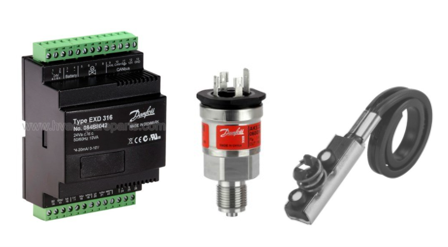
\includegraphics[width=8cm]{images/control_sensors.png}
    \caption{EXV Controller with Compatible Temperature and Pressure Sensors}
\end{figure}

\medskip
The wiring of the superheat controller will be done by Chinook Refrigeration.

\subsection{Water Pump Control}

The mass flow rate of the water is decided based on the condensing temperature selected and the coaxial condensing coil’s data sheet. In order to integrate the water circulation with the rest of the heat pump controls, a contactor is used. The contactor is used to turn the compressor on and off and is wired to it externally. Using an auxiliary switch that can be connected to the three-pole contactor, it is possible to turn the water pump on and off in tandem with the compressor. This allows both the refrigerant side and water side of the DX-SAHP to be turned on and off simultaneously. The wiring of the contactor will be done by Chinook Refrigeration.

\begin{figure}[H]
    \centering
    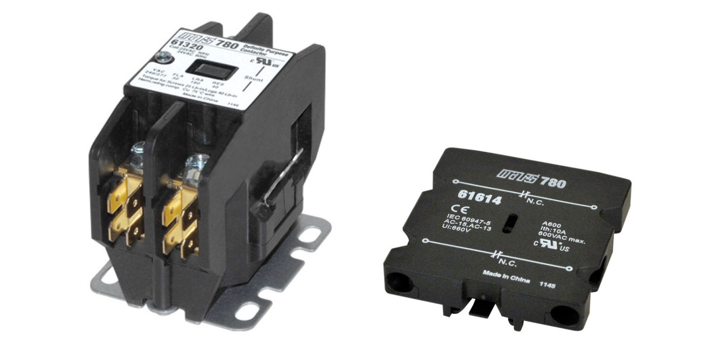
\includegraphics[width=8cm]{images/water_control.PNG}
    \caption{Three-pole Contactor (right) and Auxiliary Switch (left)}
\end{figure}

\medskip
Currently an automatic shut down of the system is missing. In future iterations, an additional control element that turns off the full system once the water in the tank is homogeneously at 55 \textdegree C can be integrated.
\chapter{Assembly Plan and Design Verification}

\section{Design and Development Plan}

The design is scheduled to be completed on March 1st, 2022, to allow for a one-month testing and verification period. The design deliverables of the project will require a full-scale working model, which does not include a system prototype. The assembly of the project will be split into 5 parts:

\medskip
\begin{enumerate}[itemsep=3mm, parsep=-1mm, label=\roman*.]
    \item Solar Thermal Collector.
    \item Piping.
    \item System Frame.
    \item Refrigerant.
    \item Data Acquisition System.
\end{enumerate}

\medskip
The Solar Thermal Collector will consist of a glass pane, absorber plate, serpentine piping manifold, and insulation, all enclosed in a plywood frame. The assembly of the thermal collector - i.e., the brazing of the serpentine manifold onto the bottom of the absorber plate - will take place concurrently with the piping fitments into the main components (i.e., compressor, condenser, expansion valve, and collector). The piping will also be welded or brazed between the components. After the frame is constructed, and the heat pump is assembled, the system can be charged with the refrigerant. As the handling and charging of refrigerants requires qualifications, three methods will be explored: 

\medskip
\begin{enumerate}[itemsep=3mm, parsep=-1mm, label=\roman*.]
    \item Support from the maintenance team at the University of Calgary will be requested to charge the system. 
    \item Support from the refrigerant training program at the Southern Alberta Institute of Technology will be requested to charge the system. 
    \item If the aforementioned strategies fail, HVAC (heating, ventilation, and air conditioning) companies will be contacted through referrals to charge the refrigerant.
\end{enumerate}

\medskip
Finally, temperature and pressure sensors for the data acquisition system will be integrated into the piping of the system to allow for the gathering of data validation metrics such as the system coefficient of performance. The temperature probes will be inserted into brazed pockets in the piping, and the pressure sensors will be screwed into the piping through specialized T-connectors.

\section{Design Verification}

To verify the design and determine the system performance, a data acquisition system was developed.

\medskip
The performance of the design can be quantified by two parameters: the $COP$ of the system and the outlet temperature of the water.

\medskip
The $COP$ of the system can be defined as:
\begin{align}
    COP = \ddfrac{Q_{out}}{W_{cycle}} = \ddfrac{\dot m (h_2 - h_3)}{\dot m (h_2 - h_1)} = \ddfrac{(h_2 - h_3)}{(h_2 - h_1)}
\end{align}

\medskip
As evidenced by Equation 4.1, the $COP$ of the system can be determined knowing the specific enthalpy of the refrigerant at certain points. Specific enthalpy at any location can be found through use of temperature and pressure measurements and the refrigeration table of R-410A [18]. As so, temperature sensors at 3 locations (1, 2, 3) and pressure sensors at 2 locations (1, 2) on Figure 4.1 below will be used to determine $COP$. The pressure sensor at 3 can be neglected under the isobaric condensation assumption. However, a temperature sensor at 3 is still necessary as it is pertinent to know and minimize the degree of subcooling at the inlet of the electronic expansion valve. Additionally, pressure transducers are approximately at least 20 times more expensive than a thermistor at any given location, so the isobaric assumption was also used for economic reasons.
In the above $COP$ equation, it was assumed that all the power input into the compressor is going into superheating the refrigerant. This in fact is not valid, as the compressor itself will hold an efficiency factor. This efficiency factor dictates how much power the compressor puts into the refrigerant, from the total power it uses.

\medskip
To evaluate this efficiency factor, the following equation will also be used to determine $COP$:
\begin{align}
    COP = \ddfrac{Q_{out}}{W_{cycle}} = \ddfrac{\dot m(h_2 - h_3)}{W_{cycle}}
\end{align}

\medskip
To determine COP using Equation 4.2, the mass flow rate of the refrigerant and the power consumption of the compressor must additionally be known. The mass flow rate of the refrigerant only needs to be measured at one location, as per the laws of continuity. A turbine flow meter will be used at location 1 for this purpose. Additionally, a power meter will be connected to the compressor to determine power usage.

\medskip
The second parameter that will be used for design verification will be the water outlet temperature. As per the design goals, the aim is to have this temperature be 55\textdegree C. A thermistor will be paced at this location to measure this parameter.

\medskip
Figure 4.1 below provides a visual guide of sensor placements in the system.

\medskip
\begin{figure}[H]
    \centering
    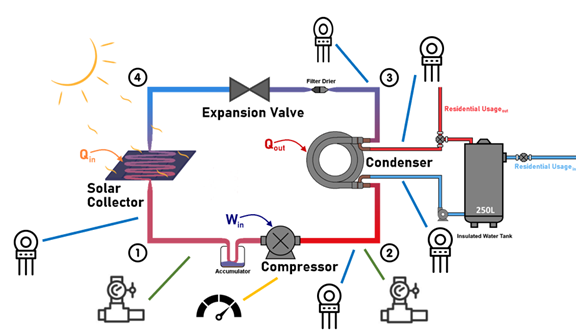
\includegraphics[width=\textwidth]{images/sensor_locations.png}
    \caption{Sensor Locations}
\end{figure}

\subsection{Data Acquisition Configuration}

To get the data outputs from the sensors, several data acquisition configurations were explored. Ultimately, an Arduino Uno was decided upon as the data acquisition device as it was the most economical option. Arduino Uno’s have only six analogs to digital converter (ADC) pins, whereas at least eight ADC pins would have been needed if all selected sensors gave analog outputs. To bypass this issue, digital thermistor sensors that could be connected to digital pins on the Arduino were chosen instead. Arduino Uno ADC pins have a maximum bit size of 12, which can affect resolution of the measurement picked up. For all the analog sensors chosen, this resulted in the smallest magnitude that could be measured being 1-2\% of the expected value. This resolution was decided to be sufficient for the needs of the data acquisition system. Table 4.1 shows a full list of sensors used. Note that the location numbering refers to schematic in Figure 4.1.

\medskip
\begin{table}[H]
\centering
\caption{List of Sensors to be used in Data Acquisition System}
\rowcolors{2}{gray!20}{white}
\begin{tabular}{|P{26mm}|P{26mm}|P{15mm}|P{27mm}|P{23mm}|P{20mm}|}
    \hline
    \rowcolor{orangeRed}
    Sensor Type & Location(s) & Accuracy & Operating Range & Power Supply & Output Type \\
    \hline
    Thermistor \cite{thermometer}            & 1, 2, 3, Water Outlet        & $\pm \SI{0.5}{\celsius}$ & $\SI{-55}{\celsius}$ to $\SI{125}{\celsius}$ & Arduino  & Digital \\
    Pressure Transducer \cite{pressure_transducer1}   & 1                            & 0.25\%                   & $0psi$ to $150psi$ & $9V$ to $30V$ DC at $<10mA$ & Analog $0V$ to $5V$ DC \\
    Pressure Transducer \cite{pressure_transducer1}   & 3                            & 0.25\%                   & $0psi$ to $1000psi$ & $9V$ to $30V$ DC at $<10mA$ & Analog $0V$ to $5V$ DC \\
    Volumetric Flow Meter \cite{pressure_transducer2} & 2                            & 3\%                      & 1L/min to 10L/min & 3.75E-5 & Amplified Square Wave \\
    Power Meter \cite{power_meter}           & Compressor Electrical Outlet & 3\%                      & 0KWH to 9999KWH & Compressor Power Supply  & Screen Display \\
    \hline
\end{tabular}
\end{table}

\medskip
All sensors will be tested and configured individually as per their respective manufacturers’ guidelines. An external power supply will be used for all sensors that require it. For more information on the different sensors that were explored, please see the Sensor Selection excel file in the Design Binder.

\medskip
To verify the design, a $COP > 2.3$ and a water outlet temperature of 55\textdegree C needs to be constantly achieved, as per design requirements. The previously described data acquisition system will assist in quantifying design verification.

\chapter{Project Management}

\section{Roles and Responsibilities of Team Members}

Each team member played a vital role in the group:

\medskip
\begin{itemize}[itemsep=3mm, parsep=-1mm]
    \item Kerwin oversaw the Project Management of the group and ensured that everything is going according to plan. He also assisted in contacting vendors and setting schedules up. 
    \item Nadia was responsible for the solar collector design and sizing. She was in charge of ensuring that the collector is functional.
    \item Jessica oversaw component matching and contacting sponsors about the component matching. 
    \item Charuka was the assembly lead. He was present during all assembly steps and oversaw much of the frame design as well.
    \item Dhruvi was in charge of the control and data acquisition system. 
    \item Edwin was the testing lead and also oversaw the condenser design.
\end{itemize}

\section{Project Schedule and Deliverables}
The major milestones that the team has completed is listed in the Table below. Please also see the Gantt Chart (Appendix B) for further detail.
\begin{table}[H]
\centering
\caption{Project Milestones}
\rowcolors{2}{gray!20}{white}
\begin{tabular}{|P{75mm}|P{75mm}|}
    \hline
    \rowcolor{orangeRed}
    Milestone & Scheduled Completion Date \\
    \hline
    First Iteration of Collector Design         & 15-Nov-21 \\
    Final Design with all Compatible Components & 01-Dec-21  \\
    Complete Bill of Materials                  & 21-Jan-22 \\
    Order all Components                        & 01-Mar-21 \\
    Prototype Assembled                         & 04-Apr-22  \\
    \hline
\end{tabular}
\end{table}


\section{Use of Project Resources and Contact Hours}
For this project, biweekly meetings with the sponsor and meetings with the faculty advisor were scheduled as needed. The team also met with advisors from Klass Mechanical for advice on a regular basis as well.

\section{Cost Overview}
A budget of \$10,000 was provided to the team to construct the prototype. The team had to be conscious of how much each component costs to remain under budget. Figure () shows a brief cost breakdown of the components that comprises the prototype.

\medskip
\begin{figure}[H]
    \centering
    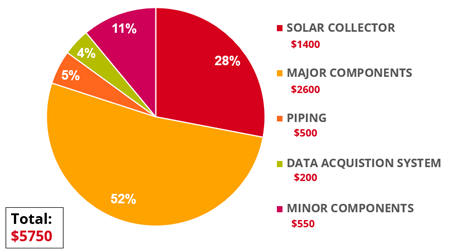
\includegraphics[width=10cm]{images/cost_breakdown.png}
    \caption{Cost Breakdown of Prototype}
\end{figure}

\medskip
Costs that are not accounted for are the costs of the expansion valve, compressor, pressure transducer and the insulation as they were provided by a sponsor.
\chapter{Closing Remarks}

\section{Summary}

DX-SAHP shows potential in replacing natural gas heaters. The parts that have been selected for the project include a flat plate collector featuring an aluminum absorber plate, a copper serpentine manifold, and a single tempered glass glazing. The system’s subcomponents, i.e., the hermetically sealed variable speed compressor, the electronic expansion valve and the condenser will be interconnected via copper tubing. Sensors have also been selected for the control of the mechanism and to enable the acquisition of data during the testing phase.

\medskip
With all the components selected, the project is on track for completion. Based on the preliminary calculations, the project is anticipated to be a success. Materials are currently being sourced for the construction of the model in the new year.

\section{Future Work}

Refer to the design binder for a complete Gantt Chart as well as a list of vendors contacted for the DX-SAHP project.

\medskip
The project was split into four phases:

\medskip
\begin{enumerate}[itemsep=3mm, parsep=-1mm, label=\roman*.]
    \item Engineering Research, Calculations, and Design.
    \item Material Acquisition.
    \item Assembly.
    \item Testing.
\end{enumerate}

\medskip
For the Fall 2021 semester, the background research, calculations, and design required to start building a working model were completed. The bill of materials is being finalized, and sponsor approval will be sought in the coming weeks. Due to COVID-19 supply chain and procurement difficulties, materials are being ordered as soon as possible to ensure project completion within the first week of April. Therefore, the timelines on the Gantt Chart are reflected to include additional contingency to ensure component delivery is met for the March 1st, 2022, assembly milestone. Finally, the testing and validation phase will take place for the remainder of the Winter 2022 semester to ensure the set design goals have been achieved.
%\chapter{LaTeX Templates}

\section{Background and Motivation}

Here is some text. Note that all of the sections and subsections will automatically be included in the table of contents. Cite your references in this manner \cite{anybody}. It is possible to emphasize text by making it \emph{italic} or \textbf{bold}.

\subsection{Subsection}

Numbering depth goes down to subsection. 

\subsubsection{Subsubsection}
Subsubsections are not numbered and do not appear in the table of contents by default. 


\section{Second section}

Figures (such as Figure \ref{Fig2}) are included like this. You'll probably want to load the \verb!graphicx! package to include images.

\begin{figure}[h]
 \caption{A description of the figure.}
 \label{Fig2}
\end{figure}


\subsection{Another subsection}

Tables (such as Table \ref{Tab2}) can be constructed and referenced like this. Footnotes\footnote{This is a footnote.} can be created like this. Make and reference numbered equations, such as equation \eqref{eq2}, like this
\begin{equation}
 \label{eq2}
 \int_{\Omega} \left(\frac{f(\gamma_1,z^{\mathcal{E}(\cos^5(x))})}{2^\ell\sqrt{g(\beta)}}\right)=\sum_{i=1}^\infty o(i\log y).
\end{equation}

\begin{table}
\centering
\begin{tabular}{|c|c|}
\hline
First column & Second column\\\hline
$a$          & Latin \\
$\aleph$     & Hebrew \\
$\alpha$     & Greek \\
7            & $1.02232134\times10^{-8}$\\
Monday       & Quidditch\\
Adam         & Dishwashing\\
\hline
\end{tabular}
\caption{A description of the table.} 

\label{Tab2}
\end{table}


%%%%%%%%%%%%%%%%%%%%%%%%%%%%%%%%%%%%%%%%%%%%%%%%%%%%%%%%%%%%%%%%%%%%%%%%%%%%%%%%%%%%%%%%%%%%%%%%%%%


% Bibliography
\thesisbibliography

%% Standard bibliography
\begin{thebibliography}{9}
\raggedright
    \bibitem{calgary_sun} O. Nag, "The Sunniest Cities in Canada," Reunion Technology Inc., 11 June 2019. [Online]. Available: \url{https://www.worldatlas.com/articles/the-sunniest-cities-in-canada.html}. [Accessed 10 December 2021].
    
    \bibitem{water_heaters} Government of Canada, "Water Heaters," Government of Canada, 4 October 2021. [Online]. Available: \url{https://www.nrcan.gc.ca/energy-efficiency/products/product-information/water-heaters/13735}. [Accessed 7 October 2021].
    
    \bibitem{stats_canada} Statistic Canada, "Appendix G Estimated number of households and average household size by domain, Canada," Statistic Canada, [Online]. Available: \url{https://www150.statcan.gc.ca/n1/pub/62f0026m/2017002/app-ann-g-eng.htm}. [Accessed 22 September 2021].
    
    \bibitem{heat_pump_water_heaters} Department of Energy, "Heat Pump Water Heaters," [Online]. Available: \url{https://www.energy.gov/energysaver/heat-pump-water-heaters}. [Accessed 3 December 2021].
    
    \bibitem{water_heater_img1} Waterheatertimer, "How to install two water heaters," [Online]. Available: \url{http://waterheatertimer.org/two-water-heaters.html}. [Accessed 6 December 2021].
    
    \bibitem{water_heater_img2} M. Bryan, "Heat Pump Water Heaters A Hot Commodity, But Not For Everyone | Northwest News Network," Northwest News Network, 7 November 2013. [Online]. Available: \url{https://www.nwnewsnetwork.org/energy/2013-11-07/heat-pump-water-heaters-a-hot-commodity-but-not-for-everyone}. [Accessed 6 December 2021].
    
    \bibitem{solar_thermal_energy} A. Smets, K. Jage, O. Isabella, R. V. Swaaij and M. Zeman, "Solar Thermal Energy," in Solar Energy: The Physics and Engineering of Photovotaic Conversion, Technologies and Systems, UIT Cambridge, pp. 497-518.
    
    \bibitem{flat_plate} C. Williams, "HeatSpring Magazine - Which is Better: Solar Thermal Flat Plate or Evacuated Tube Collectors?," HeatSpring Magazine, 10 May 2011. [Online]. Available: \url{https://blog.heatspring.com/solar-thermal-flat-plate-or-evacuated-tube-collectors/}. [Accessed 30 September 2021].
    
    \bibitem{ozone_layer} Enivronmental Protection Agency (EPA), "epa.gov," July 2015. [Online]. Available: \url{https://www.epa.gov/sites/default/files/2015-07/documents/phasing_out_hcfc_refrigerants_to_protect_the_ozone_layer.pdf}. [Accessed 3 December 2021].
    
    \bibitem{odp} United Nations Environment Programme, "Handbook for the Montreal Protocol on Substances that Deplete the Ozone Layer," United Nations Environment Programme, Nairobi, 2020.
    
    \bibitem{gwp} Environmental Protection Agency, "Understanding Global Warming Potentials," 18 October 2021. [Online]. Available: \url{https://www.epa.gov/ghgemissions/understanding-global-warming-potentials}. [Accessed 3 December 2021].
    
    \bibitem{montreal_protocol} United Nations Environment Programme, "About Montreal Protocol," [Online]. Available: \url{https://www.unep.org/ozonaction/who-we-are/about-montreal-protocol}. [Accessed 3 December 2021].

    \bibitem{hfcs} European Union, "Flourinated greenhouse gases and repealing Regulation (EC) No 842/2006," REGULATION (EU) No 517/2014 OF THE EUROPEAN PARLIAMENT AND OF THE COUNCIL of 16 April 2014 , p. 36, 2014. 

    \bibitem{ashrae_safety} American Society of Heating, Refrigerating and Air-Conditioning Engineers, "Designation and Safety Classification of Refrigerants," Standing Standard Project Committee, Atlanta, 2016.

    \bibitem{low_gwp} Air-Conditioning, Heating, \& Refrigeration Institute (AHRI), "Lower Global Warming Potential Refrigerants: Frequently Asked Questions," Arlington, 2019.

    \bibitem{low_gwp_options} M. O. McLinden, J. S. Brown, R. Brignoli, A. F. Kazakov and P. A. Domanski, "Limited options for low-global-warming-potential refrigerants," Nature Communications, p. 9, 2017.

    \bibitem{cool_prop} I. H. a. W. J. a. Q. S. a. L. V. Bell, "Pure and Pseudo-pure Fluid Thermophysical Property Evaluation and the Open-Source Thermophysical Property Library CoolProp," Industrial \& Engineering Chemistry Research, vol. 53, no. 6, pp. 2498-2508, 2014.

    \bibitem{other_compressors} K. T. A. a. K. T. Ooi, "A Review on Sliding Vane and Rolling Piston Compressors," MDPI, 21 June 2021. [Online]. Available: \url{https://www.mdpi.com/2075-1702/9/6/125/htm}. [Accessed 8 December 2021].

    \bibitem{hermetic_compressors} "Hermetic Compressors," [Online]. Available: \url{https://nptel.ac.in/content/storage2/courses/112105129/R&AC\%20Web\%20files/R&AC\%20Lecture\%202/Hyperlinks/Hermetic\%20compressors.htm}.

    \bibitem{what_hermetic_compressor} "What is Hermatically Sealed Compressor? Working, Construction \& Diagram.," Electrical Workbook, 2021 July 29. [Online]. Available: \url{https://electricalworkbook.com/hermetically-sealed-compressor/}.

    \bibitem{emerson_hermetic} EmersonAdmin, "Introducing Copeland Variable Speed Reciprocating Hermetic Compressors for Refrigeration," Emerson Climate Conversations, 9 March 2021. [Online]. Available: \url{https://emersonclimateconversations.com/2021/03/09/introducing-copeland-variable-speed-reciprocating-hermetic-compressors/}. [Accessed 6 December 2021].

    \bibitem{how_compressor_works} Bob, "How a Refrigeration Compressor Works," 2019 October 4. [Online]. Available: \url{https://www.compressorsunlimited.com/blog/how-a-refrigeration-compressor-works}.

    \bibitem{vapor_compression_refrigeration} "Vapor-compression Refrigeration," [Online]. Available: \url{https://en.wikipedia.org/wiki/Vapor-compression_refrigeration}.

    \bibitem{scroll_compressors} Bob, "What are Scroll Compressors?," Compressors Unlimited LLC, 12 March 2019. [Online]. Available: \url{https://www.compressorsunlimited.com/blog/what-are-scroll-compressors-)}.

    \bibitem{variable_speed_hermetic} D. Langenkamp, "Copeland Variable Speed Reciprocating Hermetic Compressors for Refrigeration," Emerson Climate , February 2020. [Online]. Available: \url{https://climate.emerson.com/documents/e360-variable-speed-reciprocating-hermetic-compressors-for-refrigeration.pdf}. [Accessed 6 December 2021].

    \bibitem{air_compressor} E. Waqar, "Air Compressor | What are the types of compressors?," Mechanical Boost, [Online]. Available: \url{https://mechanicalboost.com/air-compressor-types-and-applications/}. [Accessed 27 September 2021].

    \bibitem{scroll_compressor} "Scroll Compressor," LENNOX, 2021. [Online]. Available: \url{https://www.lennox.com/buyers-guide/guide-to-hvac/glossary/scroll-compressor}.

    \bibitem{what_scroll_compressor} Bob, "What are Scroll Compressors?," Compressors Unlimited International, 12 March 2019. [Online]. Available: \url{https://www.compressorsunlimited.com/blog/what-are-scroll-compressors}. [Accessed 6 December 2021].

    \bibitem{centrifugal_compressor} Nevada pneumatic, 2020. [Online]. Available: \url{https://www.nevadapneumatic.com/pro-cons-centrifugal.html}.

    \bibitem{climate_summary} G. o. Canada, "Monthly Climate Summaries," 25 November 2021. [Online]. Available: \url{https://climate.weather.gc.ca/prods_servs/cdn_climate_summary_e.html}. [Accessed 25 September 2021].

    \bibitem{exv_txv} A. M. a. D. Jamie Kitchen, "EEV's vs TXV's," 30 May 2017. [Online]. Available: \url{https://www.linkedin.com/pulse/eevs-vs-txvs-jamie-kitchen}. [Accessed 8 December 2021].

    \bibitem{txv} V. Parthan, "Thermostatic Expansion Valve| Its important concepts and 2 FAQs," LambdaGeeks, [Online]. Available: \url{https://lambdageeks.com/thermostatic-expansion-valve-concepts-and-2-faqs/}. [Accessed 8 December 2021].

    \bibitem{solar_energy_thermal_process} D, J. A. Duffie and W. A. Beckman, Solar Engineering of Thermal Processess, WIley, 2013. 
    
    \bibitem{MATLAB} Mathworks, MATLAB, 2021. 

    \bibitem{insulation} Energy Saver, "How Insulation Works," [Online]. Available: \url{https://www.energy.gov/energysaver/insulation}.

    \bibitem{heat_losses} S. H. Yoon, J.-H. Choi and K.-B. Nguyen, "Effect of working-fluid filling ratio and cooling-water flow rate on the performance of solar collector with closed-loop oscillating heat pipe.," Journal of Mechanical Science and Technology 26, January 2012. [Online]. Available: \url{https://www.researchgate.net/figure/Heat-losses-in-a-flat-plate-solar-collector_fig1_257774731}.
    
    \bibitem{thermal_insulation} Certified Commercial Property Inspectors Association, 2021. [Online]. Available: : \url{https://ccpia.org/types-of-low-slope-roof-thermal-insulation/)for}.
    
    \bibitem{insulation_design} National Mechanical Insulation Committee, "Condensation Control Calculator - Horizontal Pipe," 28 November 2016. [Online]. Available: \url{https://www.wbdg.org/guides-specifications/mechanical-insulation-design-guide/simple-calculators}.
    
    \bibitem{mineral_wool} "Mineral Wool Insulation Pros and Cons," Solar 365 the home to alternative energy, [Online]. Available: \url{http://www.solar365.com/green-homes/insulation/mineral-wool-insulation-pros-cons}. [Accessed 6 December 2021].
    
    \bibitem{emissivity} Materion, "Thermal Emissivity and Radiative Heat Transfer," Materion Performance Alloys, June 2018. [Online]. Available: \url{https://materion.com/-/media/files/alloy/newsletters/technical-tidbits/issue-no-114-thermal-emissivity-and-radiative-heat-transfer.pdf}. [Accessed 27 October 2021].
    
    \bibitem{epri} Energy.gov, "Energy Performance Ratings for Windows, Doors, and Skylights," US Department of Energy, [Online]. Available: \url{https://www.energy.gov/energysaver/energy-performance-ratings-windows-doors-and-skylights#:~:text=Solar\%20heat\%20gain\%20coefficient\%20(SHGC,the\%20greater\%20its\%20shading\%20ability.}. [Accessed 9 October 2021].
    
    \bibitem{glass_glazing} Vitro Architectural Glass, "Starphire® Glass for Exteriors," Vitro, 2021. [Online]. Available: \url{https://www.vitroglazings.com/products/low-iron-glass/starphire-ultra-clear-glass/exterior-starphire-glass/#downloads}. [Accessed 25 October 2021].
    
    \bibitem{polycarbonate_glazing} SABIC , "WLMW Polycarbonate Sheet," SABIC INNOVATIVE PLASTICS, [Online]. Available: \url{http://www.polukarbonaat.ee/juhendid/docs/cerificate/WLMW_data_sheet.pdf}. [Accessed 28 October 2021].
    
    \bibitem{low_iron_glass} JNS Glass \& Coatings, "LOW IRON GLASS – ULTRA CLEAR, STARPHIRE, OPTIWHITE," JNS, 2021. [Online]. Available: \url{https://jnsglass.com/low-iron-glass/}. [Accessed 20 October 2021].
    
    \bibitem{polycarbonate} Professional Plastics, "Polycarbonate Sheet - Standard Grade," Professional Plastics, 2021. [Online]. Available: \url{https://www.professionalplastics.com/POLYCARBONATESHEET}. [Accessed 15 October 2021].
    
    \bibitem{fiberglass} KALLITE Sales Division, "Fiberglass Solar Glazing and Greenhouse Covering," KALLITE, 2019. [Online]. Available: \url{http://www.solar-components.com/SUN.HTM}. [Accessed 10 October 2021].
    
    \bibitem{lexan} Professional Plastics, "LEXAN™ Sheet," Professional Plastics, 2021. [Online]. Available: \url{https://www.professionalplastics.com/LEXANSHEET9034}. [Accessed 12 October 2021].
    
    \bibitem{suntuf} PALRAM AMERICAS, "SUNTUF® CORRUGATED POLYCARBONATE SHEET," Palram, [Online]. Available: \url{https://www.palram.com/us/product/suntuf-diy-polycarbonate-corrugated-sheets/#1582184904168-2d0579aa-bf15}. [Accessed 21 October 2021].
    
    \bibitem{low_iron_glass_vs_regular} A. Luible, "Introduction on use of glass in modern buildings," Research Gate, April 2002. [Online]. Available: \url{https://www.researchgate.net/figure/Wave-lengths-transmission-of-regular-float-glass-and-low-iron-glass-in-comparison_fig6_37455557}. [Accessed 2 November 2021].
    
    \bibitem{plexiglass} Plastic Genius, "Plexiglass Sheets, Fiberglass, UHMW, Polycarbonate \& Engineering plastics," Plastic Genius, 20 April 2011. [Online]. Available: \url{http://www.plasticgenius.com/2011/05/infrared-and-ultraviolet-transmission.html}. [Accessed 2 November 2021].
    
    \bibitem{polycarbonate_yellowing} D. D. Priddy, "Why Do Polycarbonate Windows Sometimes Turn Yellow?," Plastic Expert Group, [Online]. Available: \url{https://www.plasticexpert.com/wp-content/uploads/2019/01/Why-Do-Polycarbonate-Windows-Turn-Yellow.pdf}. [Accessed 3 November 2021].
    
    \bibitem{thermally_conductive_materials} K. Wilson, "Top 10 Thermally Conductive Materials," Thermtest, 2018. [Online]. Available: \url{https://thermtest.com/thermal-resources/top-10-resources/top-10-thermally-conductive-materials}. [Accessed 10 October 2021].
    
    \bibitem{thermal_conductivity_of_steel} K. Wilson, "Thermal Conductivity Of Steel," Thermtest, 4 May 2021. [Online]. Available: \url{https://thermtest.com/thermal-conductivity-of-steel#:~:text=The\%20thermal\%20conductivity\%20of\%20steel,235\%20W\%2F(mK)\%20respectively.}. [Accessed 11 October 2021].
    
    \bibitem{copper_prices} Macro Trends, "Copper Prices - 45 Year Historical Chart," Macro Trends, 2021. [Online]. Available: \url{https://www.macrotrends.net/1476/copper-prices-historical-chart-data}. [Accessed 2 December 2021].
    
    \bibitem{aluminum_prices} MetalMiner, "Aluminum," MetalMiner, 2021. [Online]. Available: \url{https://agmetalminer.com/metal-prices/aluminum/}. [Accessed 2 December 2021].
    
    \bibitem{high_temp_coating} Dampney Engineered Coatings, "Industrial high-temperature protective coatings," Dampney, [Online]. Available: \url{http://www.dampney.com/Product-Line/AT/View/PID/2/Thurmalox-250}. [Accessed 15 November 2021].
    
    \bibitem{serpentine_bending} G. Winton, "Serpintine Bending in Production," 2021. [Online]. Available: \url{https://www.wintonmachine.com/serpentine-bending-in-production}.
    
    \bibitem{power_plugs} "Power Plugs and Sockets of the World.," [Online]. Available: \url{https://www.power-plugs-sockets.com/ca/canada}.
    
    \bibitem{canada_voltage} H. Chen, "What Voltage is used in Canada," [Online]. Available: \url{https://lastfiascorun.com/canada/what-voltage-is-used-in-canada.html}.
   
    \bibitem{valve_selection} Carel S.p.A, 05 August 2007. [Online]. Available: \url{file:///C:/Users/jsamb/AppData/Local/Temp/EEV\%20Valve\%20Selection\%20Criteria.pdf}.
    
    \bibitem{variable_speed_drives} "Copeland Variable Speed Reciprocating Hermetic Compressors and Drives," Emerson Climate , [Online]. Available: \url{https://climate.emerson.com/en-us/shop/1/copeland-variable-speed-hermetic-compressors-and-drives?fetchFacets=true#facet:&partsFacet:&facetLimit:&productBeginIndex:0&partsBeginIndex:0&orderBy:2&partsOrderBy:&pageView:list&minPrice:&maxPrice:&pageSize:&}. [Accessed 9 December 2021].
    
    \bibitem{exv_selection} Carel S.p.A, "Electronic Expansion Valve Selection," 05 August 2007. [Online]. Available: \url{file:///C:/Users/jsamb/AppData/Local/Temp/EEV\%20Valve\20Selection\%20Criteria.pdf}.
    
    \bibitem{water_tank_selection} Hydro Solar Innovative Energy, "All in One Buffer Tank and Indirect Water Heater 250 L - Standard Diameter Lower \& Upper Coil" Hydro Solar, [Online]. Available: \url{https://hydrosolar.ca/collections/buffer-tank-indirect-water-heater-kit/products/all-in-one-buffer-tank-and-indirect-water-heater-250-l}. [Accessed 26 November 2021].
    
    \bibitem{exv_performance} A. S. 1. (SI), "2017 Standard for Performance Rating of Expansion Valves," Air-Conditioning, Heating, and Refrigeration Institute, Arlington, 2017.
    
    \bibitem{exv_types} Danfoss, "Electric expansion valves Type ETS 6 Datasheet," August 2019. [Online]. Available: \url{https://assets.danfoss.com/documents/37229/AI227986437323en-000901.pdf}. [Accessed November 20 2021].
    
    \bibitem{fluid_mechanics} P. M.Gerhart, A. L. Gerhart and J. I. Hochstein, "Fundamentals of Fluid Mechanics Eighth Edition," WileyPlus, 2015, pp. 414 - 441.
    
    \bibitem{sporlan} Parker Hannifin Corporation, Sporlan, February 2005. [Online]. Available: \url{https://www.parker.com/literature/Sporlan/Sporlan\%20pdf\%20files/Sporlan\%20pdf\%20040/40-10-7.pdf}. [Accessed November 2021].
    
    \bibitem{accumulator} L. Molenda, "What is a Suction Accumulator?," HVAC School, 5 February 2019. [Online]. Available: \url{https://hvacrschool.com/whast-is-a-suction-accumulator/}. [Accessed 10 November 2021].
    
    \bibitem{accumulator_basics} B. Hess, "The Basics of Suction Accumulators in Home Heat Pump Systems," AC \& Heating Connect - Emerson, April 2020. [Online]. Available: \url{https://www.ac-heatingconnect.com/contractors/home-heat-pump-system-components-suction-accumulators/}. [Accessed 20 November 2021].
    
    \bibitem{sight_glass} Danfoss - Engineering Tomorrow, "Filter driers and sight glasses," Danfoss, Tuesday March 01 2011. [Online]. Available: \url{https://www.danfoss.com/en/service-and-support/case-stories/dcs/filter-driers-and-sight-glasses/}. [Accessed 15 November 2021].
    
    \bibitem{sight_glass_install} J. Marchese, "Where To Install the Liquid Line Sight Glass," The News: Air Conditioning, Heating, Refrigeration, 29 August 2020. [Online]. Available: \url{https://www.achrnews.com/articles/143707-where-to-install-the-liquid-line-sight-glass}. [Accessed 27 November 2021].
    
    \bibitem{controller} Danfoss, "Superheat controller, EKE 1D," September 2021. [Online]. Available: \url{https://assets.danfoss.com/documents/189972/AN325741271542en-000403.pdf}. [Accessed 25 November 2021].
    
    \bibitem{thermometer} Maxim, "DS18B20 Programmable Resolution 1-Wire Digital Thermometer," REV: 042208. [Online]. Available: \url{https://cdn-shop.adafruit.com/datasheets/DS18B20.pdf}. [Accessed 15 November 2021].
    
    \bibitem{pressure_transducer1} Omega, " All Stainless Steel Transducer/Transmitter Multimedia Compatibility PX309 Series," [Online]. Available: \url{https://assets.omega.com/pdf/test-and-measurement-equipment/pressure/pressure-transducers/PX309.pdf}. [Accessed 2021 28 November].
    
    \bibitem{pressure_transducer2} Vision Turbine Flow Metera, "Models BV1000, BV2000 and BV3000 for Low Viscosity and Non-Aggressive Liquids NSF/ANSI Standards 61 and 372 Certified," Februrary 2019. [Online]. Available: \url{https://assets.omega.com/spec/dynasonics_product_summary_brochure_ttm-br-01388-en_2.pdf}. [Accessed 28 November 2021].
    
    \bibitem{power_meter} "MegaPower (TM) Plug Power Meter Monitor Energy Watt Voltage Amps Meter with Electricity Usage Monitor, Reduce Your Energy Cost," [Online]. Available: \url{https://www.bestbuy.ca/en-ca/product/megapower-megapower-tm-plug-power-meter-monitor-energy-watt-voltage-amps-meter}. [Accessed 6 December 2021].
    
    \bibitem{energycalc} Direct Energy, "How Much Energy Does my Water Heater Use?," Direct Energy, 2022. [Online]. Available: \url {https://www.directenergy.com/learning-center/how-much-energy-water-heater-use}. [Accessed 25 March 2022].
    
    \bibitem{elecbill} Direct Energy, "How to Calculate Your Electric Bill," [Online]. Available: \url{https://www.directenergy.com/learning-center/how-to-calculate-electric-bill}. [Accessed 25 March 2022].
    
    \bibitem{gasrate} Gas Alberta Inc., "Gas Rates in Alberta," 2022. [Online]. Available: \url{https://www.gasalberta.com/gas-market/gas-rates-in-alberta}. [Accessed 25 March 2022].

    \bibitem{ABenergy} energyrates.ca, "Impacts on Energy Prices in Calgary, Alberta," [Online]. Available: \url{https://energyrates.ca/comparing-energy-prices-calgary-alberta/}. [Accessed 25 March 2022].
    
    \bibitem{electricheater} Home Depot, "Rheem Performance 40 Gal. Medium 6 Year 4500/4500-Watt Elements Electric Tank Water Heater XE40M06ST45U1," [Online]. Available: \url{https://www.homedepot.com/p/XE40M06ST45U1/205810725}. [Accessed 28 March 2022].
    
    \bibitem{gasheater} Home Depot, "Rheem Performance 40 Gal. Tall 6-Year 36,000 BTU Natural Gas Tank Water Heater XG40T06EC36U1," [Online]. Available: \url{https://www.homedepot.com/p/XG40T06EC36U1/205811145}. [Accessed 28 March 2022].
    
    \bibitem{PBperiod} J. Kagan, "Payback Period Definition," Investopedia, 10 March 2022. [Online]. Available: \url{https://www.investopedia.com/terms/p/paybackperiod.asp}. [Accessed 28 March 2022].
    
    \bibitem{lifeheater} Husky Air, "When Should I Replace My Hot Water Heater? Husky Knows!," 9 February 2018. [Online]. Available: \url{https://www.huskyair.com/blog/when-should-i-replace-my-water-heater/}. [Accessed 28 March 2022].
    
    \bibitem{temp_library} M. Burton, "Arduino Temperature Control Library," GitHub, 9 September 2020. [Online]. Available:  \url{https://github.com/milesburton/Arduino-Temperature-Control-Library.}. [Accessed 10 March 2022].
    
    \bibitem{temp} K. Dimitrov, "DS18B20 (Digital Temperature Sensor) and Arduino," Project Hub, 22 November 2016. [Online]. Available:  \url{https://lastminuteengineers.com/multiple-ds18b20-arduino-tutorial/.}. [Accessed 15 November 2022]
    
    \bibitem{mult_temp} LastMinuteEngineers, "Interfacing Multiple DS18B20 Digital Temperature Sensors with Arduino," LastMinuteEngineers, 2021. [Online]. Available:  \url{https://create.arduino.cc/projecthub/TheGadgetBoy/ds18b20-digital-temperature-sensor-and-arduino-9cc806.}. [Accessed 9 March 2022].
    
    \bibitem{temp_place} Direct Energy, "How Much Energy Does my Water Heater Use?," Direct Energy, 2022. [Online]. Available:   \url{https://heatpumps.co.uk/2015/06/08/temperature-sensing-with-openenergymonitor/. } [Accessed 15 October 2021].
    
    \bibitem{copeland} "Emerson Copeland zB*KA Small Scroll 3/4 to 1 1/4 HP Compressors," Emerson, [Online]. Available: \url{https://climate.emerson.com/en-ca/shop/1/copeland-sku-zb06kae-pfv-118-en-ca.} [Accessed 4 April 2022]. 
    
    \bibitem{pex_tech} "PEX Tubing Technical Specifications" PexUniverse, [Online]. Available: \url{https://www.pexuniverse.com/pex-tubing-technical-specs} [Accessed 2 April 2022]. 
    
    \bibitem{hot_water_tank} "Rheem 39 Gallon (178L) 6 Year 3kW Tank Electric Water Heater" TheHomeDepot, [Online]. Available: \url{https://www.homedepot.ca/product/rheem-39-gallon-178l-6-year-3kw-tank-electric-water-heater/1000792307} [Accessed 15 May 2022]. 
    
    \bibitem{coax_coil} "Packless 3/4 Ton Helix Copper Condenser Coil with Brackets" RefrigerativeSupply, [Online]. Available: \url{https://www.rsl.ca/Product/packless-3-4-ton-helix-copper-condenser-coil-with-brackets-coax-2076h-amt} [Accessed 15 May 2022]. 
    
    \bibitem{brazingALCU} "Brazing Aluminium and Copper," 19 March 2010. [Online]. Available: \url {https://www.aluminium-brazing.com/2010/03/19/brazing-aluminium-and-copper/.} [Accessed 4 April 2022].
    
    \bibitem{filter_drier} "EK Liquid Line Filter Drier" Emerson, [Online]. Available: \url{https://climate.emerson.com/documents/ek-liquid-line-filter-drier-capacity-table-en-4203222.pdf} [Accessed 13 March 2022].
    
    \bibitem{liquid_sight_glass} "3/8" ODF HMI-1TT3 Hermetic Sight Glass Moisture Indicator" Emerson, [Online]. Available: \url{https://www.supplyhouse.com/Emerson-Flow-Controls-065406-3-8-ODF-Hermetic-Moisture-Indicator} [Accessed  4 March 2022].
    
    \bibitem{water_valve} "V46 Pressure-Actuated Water-Regulating Valve
    Product Bulletin" JohnsonControls, [Online]. Available: \url{https://cgproducts.johnsoncontrols.com/MET_PDF/125687.PDF} [Accessed  3 March 2022].
    
    \bibitem{astro_express} "astro express 2 hot water recirculation system" Armstrong, [Online]. Available: \url{https://armstrongfluidtechnology.com/en/products/astro-express-2-hot-water-recirculation-system} [Accessed  26 March 2022].
    
    \bibitem{receiver} "Refrigeration Research 3 lb 1/4" SAE X 1/4" SAE Vertical Receiver" RefrigerativeSupply, [Online]. Available: \url{https://www.rsl.ca/Product/refrigeration-research-3-lb-1-4-sae-x-1-4-sae-vertical-receiver-1917-all} [Accessed  15 March 2022].
    
\end{thebibliography}
%%%%%%%%%%%%%%%%%%%%%%%%%%%%%%%%%%%%%%%%%%%%%%%%%%%%%%%%%%%%%%%%%%%%%%%%%%%%%%%%%%%%%%%%%%%%%%%%%%%


%% Appendices
\appendix

\chapter{Appendix A: Gantt Chart}

\begin{figure}[H]
    \centering
    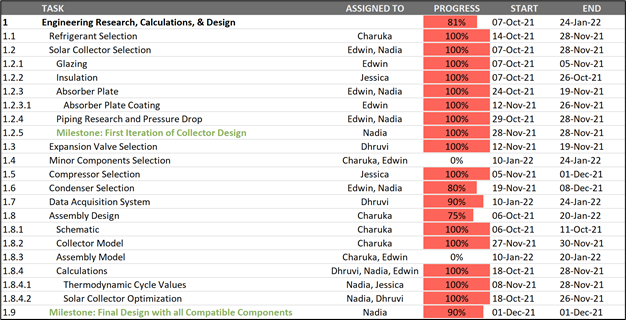
\includegraphics[width=15cm]{images/gantt1.png}
\end{figure}
\begin{figure}[H]
    \centering
    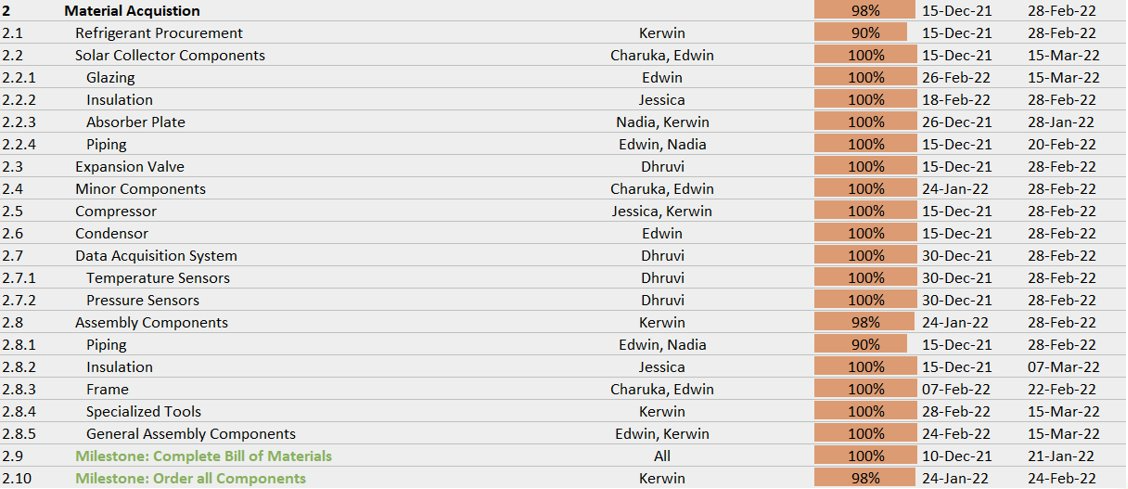
\includegraphics[width=15cm]{images/gantt2.png}
\end{figure}
\begin{figure}[H]
    \centering
    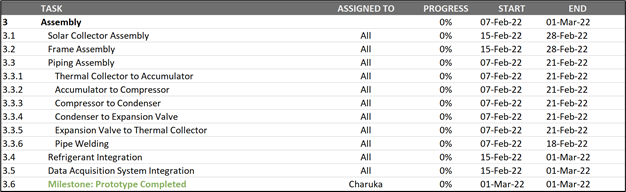
\includegraphics[width=15cm]{images/gantt3.png}
\end{figure}
\begin{figure}[H]
    \centering
    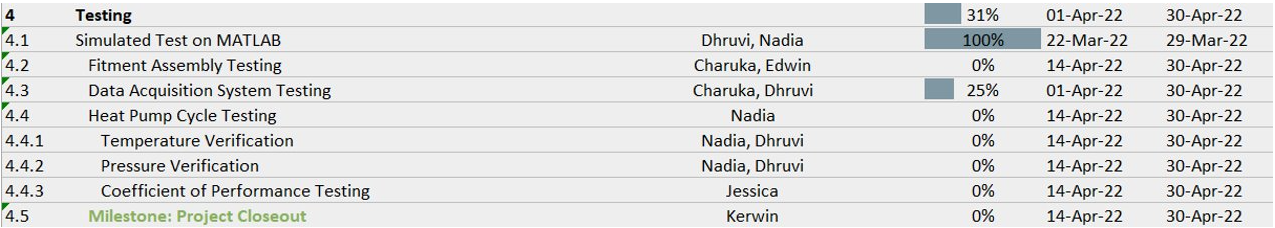
\includegraphics[width=15cm]{images/gantt4.png}
\end{figure}



\chapter{Appendix B: Gantt Chart}

\begin{figure}[H]
    \centering
    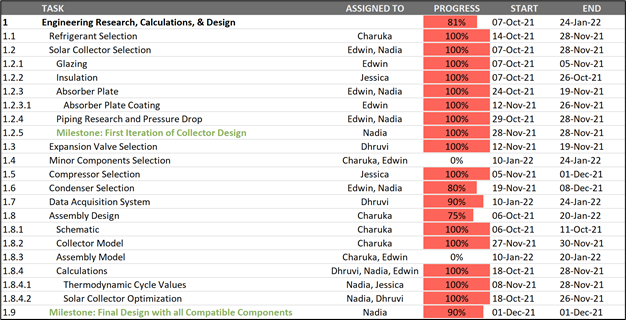
\includegraphics[width=15cm]{images/gantt1.png}
\end{figure}
\begin{figure}[H]
    \centering
    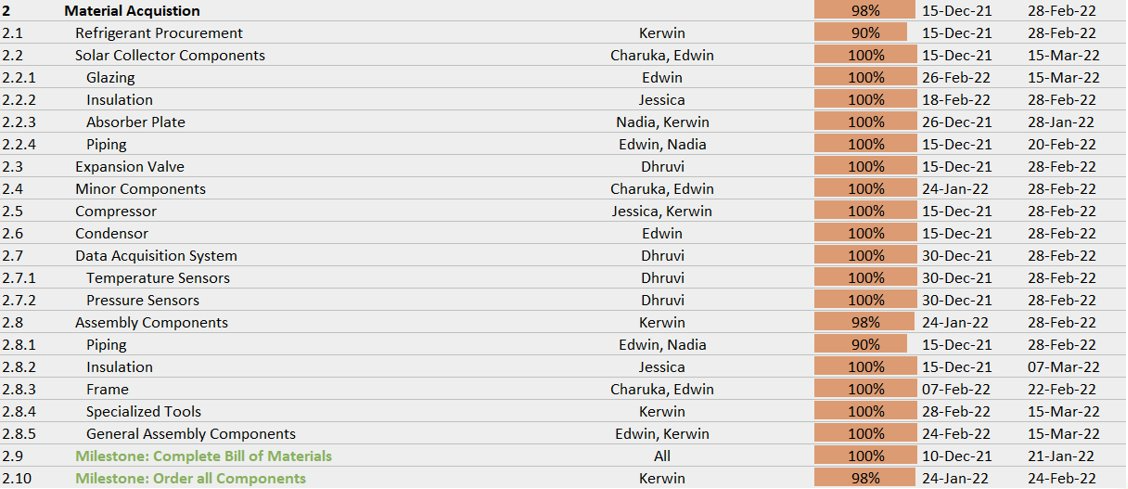
\includegraphics[width=15cm]{images/gantt2.png}
\end{figure}
\begin{figure}[H]
    \centering
    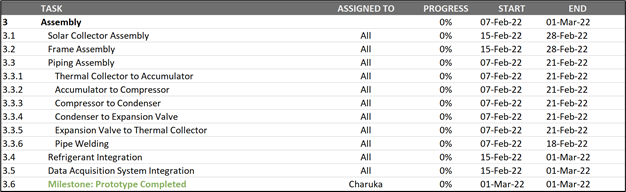
\includegraphics[width=15cm]{images/gantt3.png}
\end{figure}
\begin{figure}[H]
    \centering
    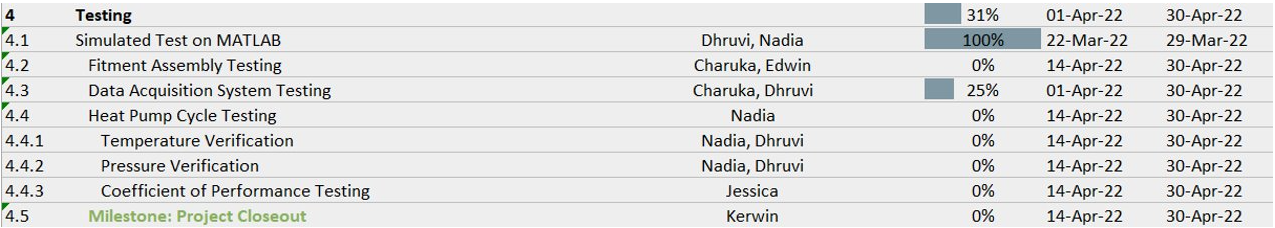
\includegraphics[width=15cm]{images/gantt4.png}
\end{figure}



%%%%%%%%%%%%%%%%%%%%%%%%%%%%%%%%%%%%%%%%%%%%%%%%%%%%%%%%%%%%%%%%%%%%%%%%%%%%%%%%%%%%%%%%%%%%%%%%%%%


% End of Document
\end{document}
